%%%%%%%%%%%%%%%%%%%%%%%%%%%%%%%%%%%%%%%%%%%%%%%%%%%%%%%%%%%%%%%%%%%%%%%%%%%%%%%%
% thesis.tex: Primary TeX control file for thesis.
%%%%%%%%%%%%%%%%%%%%%%%%%%%%%%%%%%%%%%%%%%%%%%%%%%%%%%%%%%%%%%%%%%%%%%%%%%%%%%%%
\documentclass[11pt, oneside]{mnthesis}
\draft
\usepackage{epsfig} % Allows the inclusion of eps files
\usepackage{epic} % Enhanced picture mode
\usepackage{eepic} % Extensions for epic
\usepackage{units} % SI unit typesetting
\usepackage{url} % URL handling
\usepackage{longtable} % Tables that continue onto multiple pages
\usepackage{mathrsfs} % Support for \mathscr script
\usepackage{multirow} % Span rows in tables
\usepackage{bigstrut} % Space struts in tables up and down
\usepackage{amssymb} % AMS math symbols and helpers
\usepackage{graphicx} % Enhanced graphics support
\usepackage{setspace} % Adjust spacing in captions, single by default
\usepackage{xspace} % Automatically adjusting space after macros
\usepackage{amsmath} % \text, and other math formatting options
\usepackage{siunitx} % \num{} formatting and SI unit formatting
\usepackage{booktabs} % Enhanced tables with \toprule, etc.
\usepackage{hyperref} % Add clickable links to other parts of the document
\usepackage[noabbrev]{cleveref} % Automatically determine \cref type

% Configure the siunitx package
\sisetup{
    group-separator = {,}, % Use , to separate groups of digits, like 12,345
    list-final-separator = {, and } % Always use the serial comma in \SIlist
}

% Configure the cleveref package
\newcommand{\creflastconjunction}{, and } % Always use the serial comma

\linespread{1.0}
% Compile only the chapters listed here
\includeonly{
preliminaries/title,
chapters/adapter_synthesis,
chapters/path_merging_connection,
chapters/java_ranger,
chapters/program_repair,
chapters/conclusion,
%chapters/app_glossary,
%chapters/adapter_synthesis_appendix
}

%begin adapter_synthesis preamble
\usepackage{listings}
\usepackage{color}
\usepackage{amsmath,amssymb}
% Workaround for compatibility between older (e.g., Ubuntu 12.04)
% versions of algorithm2e and the ACM template
% https://depinfi.wordpress.com/2012/11/26/using-algorithm2e-in-acm-template/
% Commented out in favor of just keeping the 14.04 version of algorithm2e
% in the repository.
%\makeatletter
%\newif\if@restonecol
%\makeatother
%\let\algorithm\relax
%\let\endalgorithm\relax
\usepackage{algorithm2e}
\usepackage{wrapfig}


\usepackage[nounderscore]{syntax}

\usepackage{newfloat}

\usepackage{todonotes}
\DeclareGraphicsExtensions{.pdf,.jpeg,.png}


\usepackage{float}
% Physics constants
\newcommand{\C}{{\mathrm{c}}}

% Add space between rows of tables
\newcommand{\spacerows}[1]{\renewcommand{\arraystretch}{#1}}

% Define a better looking eV by moving the V slightly left
\DeclareSIUnit\electronvolt{e\hspace{-0.08em}V}

\newcommand*{\permcomb}[4][0mu]{{{}^{#3}\mkern#1#2_{#4}}}
\newcommand*{\perm}[1][-3mu]{\permcomb[#1]{P}}
\newcommand*{\comb}[1][-1mu]{\permcomb[#1]{C}}

\newcommand{\widthfactor}{0.7}
%    \usepackage{lineno}
% http://tex.stackexchange.com/questions/7996/lineno-and-syntax-package-incompatibilities
%    \makeatletter
%    \def\gr@implitem<#1> #2 {%
%     \sbox\z@{\hskip\labelsep\grammarlabel{#1}{#2}}%
%      \strut\@@@par% lineno.sty redefines \@@par which was in the original code
%     \vspace{-\parskip}%
%      \vspace{-\baselineskip}%
%      \hrule\@height\z@\@depth\z@\relax%
%      \item[\unhbox\z@]%
%      \catcode`\<\active%
%    }
%    \makeatother

\lstset{language=C}

\lstdefinestyle{nonumbers}
{numbers=none}

\definecolor{mygreen}{rgb}{0,0.4,0}
\definecolor{mygray}{rgb}{0.5,0.5,0.5}
\definecolor{mymauve}{rgb}{0.58,0,0.82}
\lstset{ %
backgroundcolor=\color{white},   % choose the background color; you
%must add \usepackage{color} or \usepackage{xcolor}
basicstyle=\ttfamily\small,        % the size of the fonts that are used
%for the code
basewidth = {.5em, 0.5em},
%breakatwhitespace=false,         % sets if automatic breaks should
%only happen at whitespace
breaklines=true,                 % sets automatic line breaking
captionpos=b,                    % sets the caption-position to bottom
commentstyle=\color{mygreen},    % comment style
deletekeywords={...},            % if you want to delete keywords from
%the given language
escapeinside={\%*}{*)},          % if you want to add LaTeX within
%your code
extendedchars=true,              % lets you use non-ASCII characters;
%for 8-bits encodings only, does not work with UTF-8
frame=single,	                   % adds a frame around the code
keepspaces=true,                 % keeps spaces in text, useful for
%keeping indentation of code (possibly needs columns=flexible)
keywordstyle=\color{blue},       % keyword style
language=C,                 % the language of the code
otherkeywords={reg8\_t,reg64\_t},           % if you want to add more keywords to
%the set
numbers=left,                    % where to put the line-numbers;
%possible values are (none, left, right)
numbersep=5pt,                   % how far the line-numbers are from
%the code
numberstyle=\tiny\color{black}, % the style that is used for the
%line-numbers
rulecolor=\color{black},         % if not set, the frame-color may be
%changed on line-breaks within not-black text (e.g. comments (green
%here))
showspaces=false,                % show spaces everywhere adding
%particular underscores; it overrides 'showstringspaces'
%  showstringspaces=false,          % underline spaces within strings
%only
showtabs=false,                  % show tabs within strings adding
%particular underscores
stepnumber=1,                    % the step between two line-numbers.
%If it's 1, each line will be numbered
stringstyle=\color{mymauve},     % string literal style
tabsize=2,	                   % sets default tabsize to 2 spaces
%  title=\lstname                   % show the filename of files included
%with \lstinputlisting; also try caption instead of title
literate={->}{$\rightarrow$}{2}
{α}{$\alpha$}{1}
{δ}{$\delta$}{1}
}

% declare the floating environment {Grammar}
% this will also define \listofGrammars:
\DeclareFloatingEnvironment[
% the file extension for the file used to create the list:
fileext   = logr,% don't use log here!
% the heading for the list:
listname  = {List of Grammars},
% the name used in captions:
name      = Grammar,
% the default floating parameters if the environment is used
% without optional argument:
placement = htp
]{Grammar}
%end adapter_synthesis preamble

%begin Java Ranger preamble
\usepackage{booktabs} % For formal tables
\usepackage{listings}
\usepackage{url}
\usepackage{color}
\usepackage{authblk}
\usepackage{graphicx}
\usepackage{subcaption}
\captionsetup{compatibility=false}
%end Java Ranger preamble


\begin{document}
\bibliographystyle{hunsrt} % style of bibliography
%%%%%%%%%%%%%%%%%%%%%%%%%%%%%%%%%%%%%%%%%%%%%%%%%%%%%%%%%%%%%%%%%%%%%%%%%%%%%%%%

%%%%%%%%%%%%%%%%%%%%%%%%%%%%%%%%%%%%%%%%%%%%%%%%%%%%%%%%%%%%%%%%%%%%%%%%%%%%%%%%
% Title and other sections that come before the body of the document
%%%%%%%%%%%%%%%%%%%%%%%%%%%%%%%%%%%%%%%%%%%%%%%%%%%%%%%%%%%%%%%%%%%%%%%%%%%%%%%%
%%%%%%%%%%%%%%%%%%%%%%%%%%%%%%%%%%%%%%%%%%%%%%%%%%%%%%%%%%%%%%%%%%%%%%%%%%%%%%%%
% title.tex - Set up the beginning of thesis.
%%%%%%%%%%%%%%%%%%%%%%%%%%%%%%%%%%%%%%%%%%%%%%%%%%%%%%%%%%%%%%%%%%%%%%%%%%%%%%%%

% Uncomment to turn on draft mode, which changes the title page to have a draft
% label and date of compilation
%\draft

% Set the type of thesis
\phd % use if for a Ph.D. dissertation
%\ms % use if for a Master of Science thesis

% Set the title and your name. Remember that the guidelines state:
%
% "The title of the thesis must not contain chemical or mathematical formulas,
% symbols, superscripts, subscripts, Greek letters, or other non-standard
% characters; words must be substituted."
\title{\bf Thesis Proposal}
\author{Vaibhav Bhushan Sharma}
% Advisor name, put co-advisors here as well separated by commas
\director{Stephen McCamant}

% Specify the month and year; if commented out then these default to the
% current month and year
\submissionmonth{Dec}
\submissionyear{2018}

% Pages after the title page
\abstract{%%%%%%%%%%%%%%%%%%%%%%%%%%%%%%%%%%%%%%%%%%%%%%%%%%%%%%%%%%%%%%%%%%%%%%%%%%%%%%%%
% abstract.tex: Abstract
%%%%%%%%%%%%%%%%%%%%%%%%%%%%%%%%%%%%%%%%%%%%%%%%%%%%%%%%%%%%%%%%%%%%%%%%%%%%%%%%
Abstract
%%%%%%%%%%%%%%%%%%%%%%%%%%%%%%%%%%%%%%%%%%%%%%%%%%%%%%%%%%%%%%%%%%%%%%%%%%%%%%%%
}

% Copyright: Uncomment one of the following:
\copyrightpage       % Full copyright
%\copyrightpageccby   % Full copyright with Creative Commons CC-BY 4.0 license
%\copyrightpageccbysa % Full copyright with Creative Commons CC-BY-SA 4.0 license

% Acknowledgments and dedication
\acknowledgements{\input{preliminaries/acknowledge}}
\dedication{\input{preliminaries/dedication}}

% Use a special preface
%\extra{\input{preface}}

% The \beforepreface command actually causes insertion of the title,
% abstract, signature, and copyright pages into the new document.
\beforepreface

% Define the text to go before the table of contents
\figurespage
\tablespage

% The \afterpreface command actually causes insertion of the
% contents, list of figures, etc. into the new document.
\afterpreface
%%%%%%%%%%%%%%%%%%%%%%%%%%%%%%%%%%%%%%%%%%%%%%%%%%%%%%%%%%%%%%%%%%%%%%%%%%%%%%%%

%%%%%%%%%%%%%%%%%%%%%%%%%%%%%%%%%%%%%%%%%%%%%%%%%%%%%%%%%%%%%%%%%%%%%%%%%%%%%%%%

%%%%%%%%%%%%%%%%%%%%%%%%%%%%%%%%%%%%%%%%%%%%%%%%%%%%%%%%%%%%%%%%%%%%%%%%%%%%%%%%
% Now lets include the body of the document...
%%%%%%%%%%%%%%%%%%%%%%%%%%%%%%%%%%%%%%%%%%%%%%%%%%%%%%%%%%%%%%%%%%%%%%%%%%%%%%%%
%%%%%%%%%%%%%%%%%%%%%%%%%%%%%%%%%%%%%%%%%%%%%%%%%%%%%%%%%%%%%%%%%%%%%%%%%%%%%%%%
% intro.tex: Introduction to the thesis proposal
%%%%%%%%%%%%%%%%%%%%%%%%%%%%%%%%%%%%%%%%%%%%%%%%%%%%%%%%%%%%%%%%%%%%%%%%%%%%%%%%
\chapter{Introduction}
\label{intro_chapter}
%%%%%%%%%%%%%%%%%%%%%%%%%%%%%%%%%%%%%%%%%%%%%%%%%%%%%%%%%%%%%%%%%%%%%%%%%%%%%%%%

\begin{itemize}

\item Chapter 1 presents adapter synthesis.

\item Chapter 2 presents the need to have path-merging with adapter synthesis.

\item Chapter 3 presents a path-merging approach integrated symbolic execution of Java bytecode.

\item Chapter 4 describes an application of adapter synthesis towards binary program repair.

\end{itemize}
%%%%%%%%%%%%%%%%%%%%%%%%%%%%%%%%%%%%%%%%%%%%%%%%%%%%%%%%%%%%%%%%%%%%%%%%%%%%%%%%


%Base Chapters
%%%%%%%%%%%%%%%%%%%%%%%%%%%%%%%%%%%%%%%%%%%%%%%%%%%%%%%%%%%%%%%%%%%%%%%%%%%%%%%%
%adapter_synthesis.tex: Chapter on adapter synthesis
%%%%%%%%%%%%%%%%%%%%%%%%%%%%%%%%%%%%%%%%%%%%%%%%%%%%%%%%%%%%%%%%%%%%%%%%%%%%%%%%
\chapter{Finding Substitutable Binary Code By Synthesizing Adapters}
\label{adapter_synthesis_chapter}
%%%%%%%%%%%%%%%%%%%%%%%%%%%%%%%%%%%%%%%%%%%%%%%%%%%%%%%%%%%%%%%%%%%%%%%%%%%%%%%%
%\documentclass[journal]{IEEEtran}





\section{Introduction}
%
Given the large corpus of software available today to an average programmer
to reuse, it is desirable to reuse well-tested, bug-free chunks of
code that implement some required functionality.
%
Finding such code can be difficult to automate, and there is no
guarantee that the code found by such a search will have the exact
interface the programmer intends to use. 
%
At such times, programmers find themselves writing wrapper code and
creating unit tests to check if the wrapped code works as they intended.
%
In this paper, we improve upon a previously presented technique~\cite{icst-adaptersynth} that automates the process of
finding functions that match the behavior specified by an existing
function, while also synthesizing the necessary wrapper needed to handle 
interface differences between the original and discovered functions.
%
Use cases for our improved technique include replacing insecure dependencies of off-the-shelf libraries with bug-free variants, reverse engineering binary-level functions by comparing their behavior to known implementations, and locating multiple versions of a function to be run in parallel to provide security through diversity~\cite{BorckBDHHJSS2016}.

Our technique works by searching for a wrapper that can be added around one function's interface to make it equivalent to another function.
%
We consider wrappers that transform function arguments and return values.
%
For example, Listing~\ref{lst:isalpha} shows implementations of the \textit{isalpha} predicate, which checks if a character is a letter, in two commonly-used libraries.
%
Both implementations follow the ISO C standard specification of the \textit{isalpha} function, but the glibc implementation signifies the input is a letter by returning 1024, while the musl implementation returns 1 in that case.
%
The glibc implementation can be adapted to make it equivalent to the musl implementation by replacing its return value, if non-zero, by 1 as shown by the \textit{adapted\_isalpha} function.
%
This illustrates the driving idea of our approach: to check whether two functions, $f_1$ and $f_2$, have different interfaces to the same functionality, we can search for a wrapper that allows $f_1$ to be substituted by $f_2$.

We refer to the function being wrapped around as the {\em reference} function and the function being emulated as the {\em target} function.
%
In the example above, the reference function is \textit{glibc\_isalpha} and the target function is \textit{musl\_isalpha}.
%
We refer to the wrapper code automatically synthesized by our tool as an {\em adapter}.
%
Our adapter synthesis tool searches in the space of all possible adapters allowed by a specified adapter family for an adapter that makes the behavior of the reference function $f_2$ equivalent to that of the target function $f_1$.
%
We represent that such an adapter exists by the notation $f_1 \leftarrow f_2$.
%
Note that this adaptability relationship is not symmetric: $f_1 \leftarrow f_2$ does not imply $f_2 \leftarrow f_1$. 
%
%In the \textit{isalpha} example, the other direction of adapter could be implemented by multiplying the musl implementation\rq s return value with 1024, but in general only one direction of adaptation may be possible.
%
To efficiently search for an adapter, we use counterexample guided inductive synthesis~(CEGIS)~\cite{Solar-LezamaTBSS2006}.
%
An adapter family is represented as a formula for transforming values controlled by parameters: each setting of these parameters represents a possible adapter.
%
Each step of CEGIS allows us to conclude that either a counterexample exists for the previously hypothesized adapter, or that an adapter exists for all previously found tests.
%
We use binary symbolic execution both to generate counterexamples and to find new candidate adapters; the symbolic execution engine internally uses a satisfiability modulo theories~(SMT) solver.
%
We also implement adapter search using a randomly-ordered enumeration of all possible adapters.
%
We always restrict our search to a specified finite family of adapters.
\lstinputlisting[caption={musl and glibc implementations of the \textit{isalpha} predicate and a wrapper around the glibc implementation that makes it equivalent to the musl implementation},
label={lst:isalpha}, style=nonumbers]{chapters/adapter_synthesis/code_samples/musl_glibc.c}
%
We implement adapter synthesis to adapt around inputs and outputs in registers and memory.
%
We demonstrate the use of adapter synthesis for the following applications.
%
\begin{itemize}
\item We demonstrate the use of adapter synthesis for adaptably substituting
a buggy function with its bug-free variant by finding 
adaptable equivalence modulo a bug.
%
\item We demonstrate substitution of RC4 key structure
setup and encryption functions in mbedTLS~(formerly PolarSSL) and
OpenSSL by means of synthesizing adapters between their interfaces. 
%
\item We present an intra-library evaluation of adapter synthesis by
evaluating two of our adapter families on more than 13,000 pairs of
functions from the GNU C library.
%
\item We demonstrate the use of adapter synthesis for reverse engineering at
scale using binary symbolic execution-based adapter synthesis.
%
We show that code fragments in a ARM-based 3rd party firmware image for
the iPod Nano 2g device can be adaptably substituted by reference
functions written for the VLC media player~\cite{vlc}.
%
In this evaluation, we complete more than 1.17 million synthesis tasks,
with each synthesis task navigating an adapter search space of more than
1.353 x $10^{127}$ adapters.
%
%Enumerating this search space concretely would take an infeasible amount of time~($10^{14}$ years).
%
We find our adapter synthesis implementation finds several instances of reference functions in the firmware image.
\end{itemize}

The rest of this chapter is organized as follows.
%
Section~\ref{sec:adapter_synthesis} presents our algorithm for adapter synthesis and describes our adapter families.
%
Section~\ref{sec:implementation} describes our implementation, and
Section~\ref{sec:evaluation} presents examples of application of adapter synthesis, large-scale evaluations, and a comparison of two adapter search implementations.
%
Section~\ref{sec:discussion} discusses limitations and future work,
Section~\ref{sec:related-work} describes related work, and
Section~\ref{sec:conclusion} concludes.
% 
%  Previous introduction written by Stephen  
%
%    It is commonly observed that of the large amount of software being
%    written, there are many instances of repeated functionality.
%    %
%    Such repetition can occur both within one program and between separate
%    programs, and while some duplication occurs by syntactic copying
%    (``cut and paste''), in other cases functionally equivalent code is
%    developed independently by different developers.
%    %
%    Duplication can sometimes be a burden (because it bloats code and
%    allows bugs fixed in one version to persist in another), but it can
%    also be a resource that makes other useful tasks possible.
%    %
%    For instance diverse implementations of the same functionality can be
%    used for fault tolerance, or if implementations differ in performance
%    we can optimize a program by replacing a slower function with a faster
%    one.
%    
%    The most familiar techniques for finding code duplication examine
%    program source code, and search for code segments that are the same at
%    the level of code syntax (syntactic clones).
%    %
%    But for many applications we wish to find functions that have the same
%    behavior even if their implementations are syntactically different
%    (semantic clones).
%    %
%    For security applications, or when operating on legacy software, it
%    can also be desirable to find clones even when some or all of the
%    software involved is available only it its final executable
%    (``binary'') form.
%    %
%    A semantic rather than a syntactic approach is also natural for
%    binaries because the compilation process can introduce many kinds
%    instruction-level variation.
%    %
%    With these applications in mind we explore techniques for finding
%    semantically-equivalent code at the binary level.
%    
%    The application that originally motivated us is using semantically
%    equivalent code segments to make variants of a program with
%    implementation diversity that can help it to withstand faults or even
%    malicious attack.
%    %
%    This can be particularly effective if multiple diverse variants are
%    executed together and checked for
%    divergence~\cite{Cox:2006:NSS:1267336.1267344}.
%    %
%    Such a defense is stronger if the variants are more semantically
%    diverse, but most techniques that automatically produce variant
%    executables from a single source program affect only low-level
%    features like memory layout~\cite{Larsen:2014:SAS:2650286.2650803},
%    and so provide protection only against low-level attacks.
%    %
%    Finding usable alternative implementations in existing code bases is a
%    promising direction for discovering semantic diversity that can
%    provide more robust protection~\cite{BorckBDHHJSS2016}.
%    
%    A challenge for finding semantic equivalence is that code we would
%    intuitively consider to implement the same functionality might have a
%    different interface, especially if it was developed independently.
%    %
%    (For now we concentrate on code segments that implement functions, so
%    the interfaces we consider are function interfaces.)
%    %
%    An equivalence checking technique that was only able to find
%    implementations with exactly the same interface would miss many
%    semantic clones.
%    %
%    Programmers typically bridge incompatible function interfaces by
%    writing wrapper code that we call an {\em adapter}: a function that
%    implements one interface in terms of another one by making small
%    changes such as copying or reformatting data, or rearranging function
%    arguments.
%    %
%    When we can write an adapter that wraps a function $f_2$ to make it
%    equivalent to a function $f_1$, we write $f_1 \leftarrow f_2$.
%    %
%    The function $f_2$ which is inside the wrapper function we call the
%    {\em inner function}, while the function $f_1$ whose functionality we
%    want to emulate we refer to as the {\em target function}.
%    %
%    The combination of the adapter and the inner function, which is
%    semantically equivalent to the target function, we call the {\em outer
%      function}.
%    
%    This suggests that we would like to consider two functions to be
%    semantically equivalent whenever such an adapter function might be
%    written to replace one with the other.
%    %
%    Because such adapters have a stylized form and the specification in
%    terms of function equivalence is precise, we observe that we can turn
%    this intuition into an automated approach by applying program
%    synthesis.
%    %
%    Given a pair of functions, our system searches over a space of
%    possible adapter functions until it either finds an adapter that makes
%    the outer function equivalent to the target function, or proves that
%    no such adapter exists.
%    %
%    Though this basic approach could be applied equally well to source
%    code or binary code, we implement it using binary-level symbolic
%    execution to increase its applicability, including to systems written
%    using a mixture of C and assembly language.
%    
%    It would be challenging to find a correct adapter in a single search,
%    since the spaces of function inputs and possible adapters are in
%    general both large, and an adapter must work for all inputs.
%    %
%    (From a logical perspective, this corresponds to the fact that the
%    full problem has a quantifier alternation: we seek to show that {\em
%      there exists} an adapter which works {\em for all} inputs.)
%    %
%    To make the search more tractable, we use the technique of
%    counterexample-guided inductive synthesis (CEGIS) to split it into an
%    alternation of two kinds of search.
%    %
%    Rather than demanding an adapter that works over all inputs from the
%    start, our algorithm grows a finite set of test cases, searching at
%    each step for an adapter that works for the current set of test cases,
%    and then checking whether that particular adapter works for all
%    inputs.
%    %
%    Both of these simpler search steps can be implemented with symbolic
%    execution and quantifier-free SMT (satisfiability modulo theories)
%    solving.
%    
%    A key factor in making this approach practical is choosing a space of
%    possible adapters which is large enough to find many related
%    functions, but limited enough that synthesis is tractable.
%    %
%    So we investigate a number of different adapter grammars and
%    illustrate them with examples.
%    %
%    We have implemented out approach on top of an existing binary symbolic
%    execution system, and we evaluate it with a large-scale case study
%    looking for semantically-adaptable function pairs in the standard C
%    library used on Linux (eglibc 2.19 from Ubuntu 14.04).
%    
%    The rest of this paper is organized as follows.
%    %
%    Section~\ref{sec:overview} describes more specifically the kind of
%    adapters we search for, with examples.
%    %
%    Section~\ref{sec:adapter_synthesis} gives our algorithm for adapter
%    synthesis and describes our adapter grammar.
%    %
%    Section~\ref{sec:implementation} describes our implementation, and
%    Section~\ref{sec:evaluation} presents the C library case study.
%    %
%    Section~\ref{sec:discussion} discusses limitations and future work,
%    Section~\ref{sec:related-work} describes related work, and
%    Section~\ref{sec:conclusion} concludes.


%\input{overview}

\section{Adapter Synthesis}
\label{sec:adapter_synthesis}
%
\subsection{Algorithm for Adapter Synthesis}
%
The idea behind CEGIS is to alternate between synthesizing candidate expressions and checking whether those expressions meet a desired specification. 
%
When a candidate expression fails to meet the specification, a counterexample is produced to guide the next synthesis attempt.
%
In our case, the expressions to be synthesized are adapters that map inputs of the target function to inputs of the reference function and outputs of the reference function to outputs of the target function in such a way that the behavior of the two matches. 
%
Our specification for synthesis is provided by the behavior of the target function and we define counterexamples to be inputs on which the behavior of the reference function and target function differ for a given adapter.
%
Our adapter synthesis algorithm is summarized in Figure~\ref{fig:adapter_synthesis}.
%
\begin{figure}[]
\centering
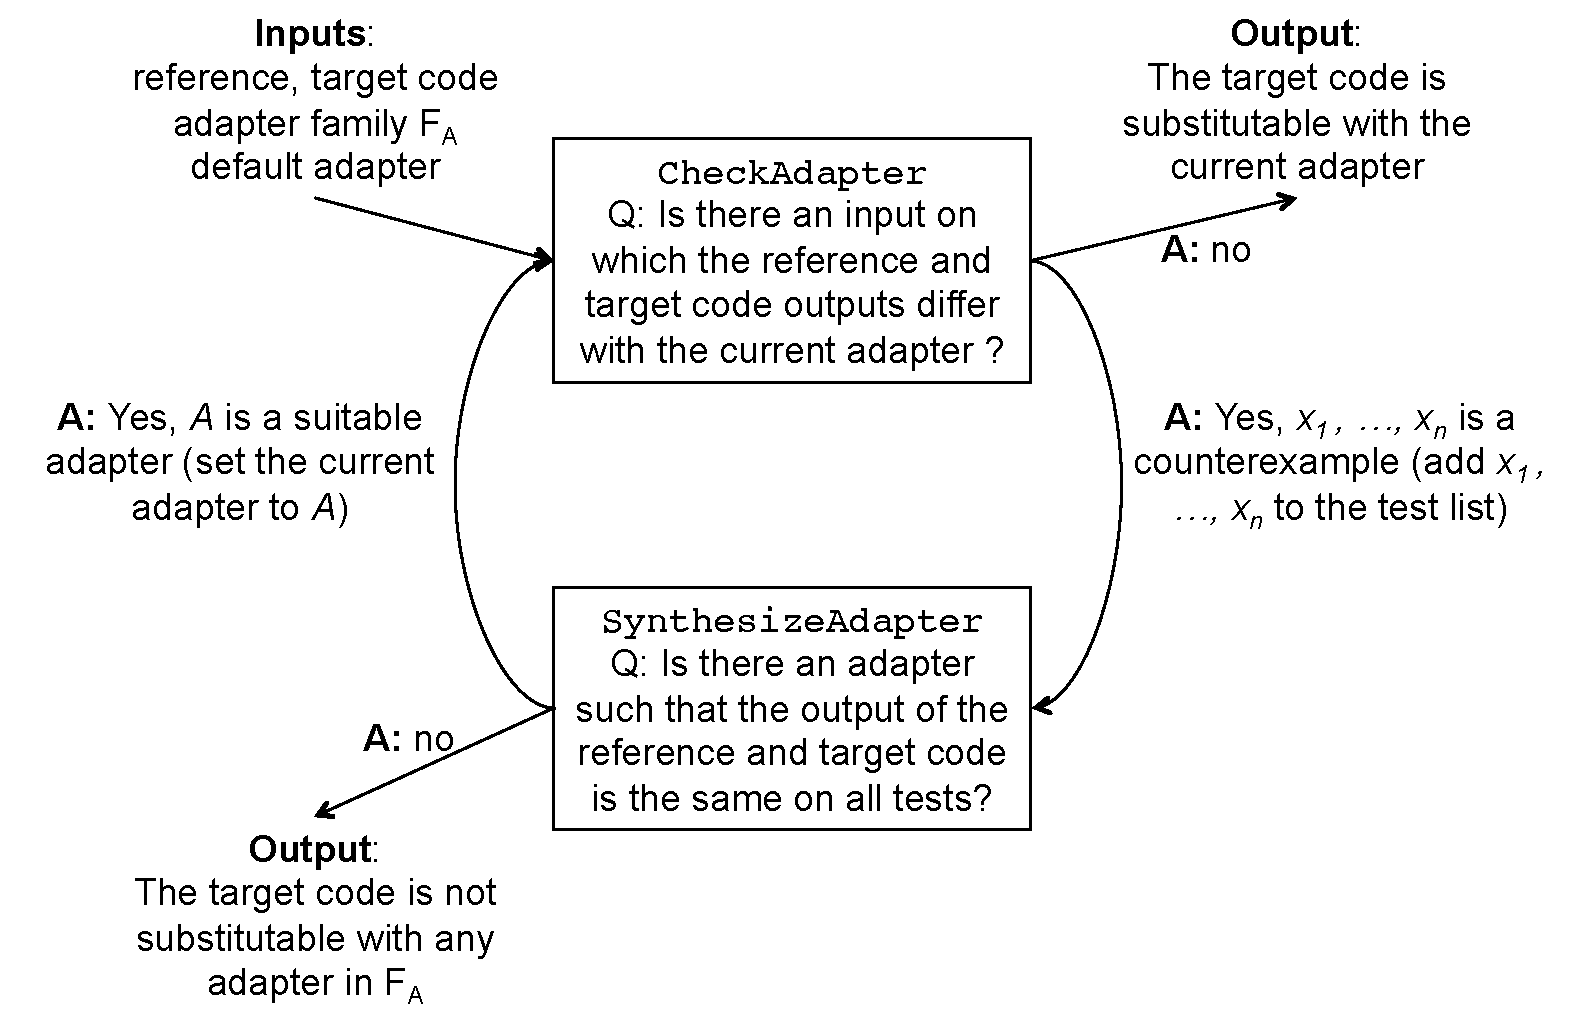
\includegraphics[scale=0.42]{chapters/adapter_synthesis/figures/adapter_synthesis_diagram_v3}
\caption{Counterexample-guided adapter synthesis}
\label{fig:adapter_synthesis}
\end{figure}
%
%More expressive adapters allow for equivalence between more function pairs, but may considerably increase the time required to find a correct adapter.
%
%The adapter grammars we present in the next section represent a trade-off between the desires for generality of adapters and reasonable synthesis performance.
%
As shown in Figure~\ref{fig:adapter_synthesis}, our algorithm takes as input the reference function, the target function, and an adapter family $F_A$. 
%
The algorithm begins with a default adapter and an empty test list.
%
In our implementation, as a default adapter we often use the ``zero adapter,'' which sets every input and output of the reference function to the constant value 0.
%
Until a correct adapter is found or no new adapter can be synthesized, a new counterexample is added to the test list, and any subsequently generated candidate adapters must satisfy all tests in the list.
%
The output of adapter synthesis is either input and output adapters that allow the target function to be substituted by the adapted reference function or an indication that achieving substitutability is not possible using the specified adapter family $F_A$.
%
Our algorithm is guaranteed to terminate if the space of adapters allowed by $F_A$ is finite~\cite{Solar-LezamaTBSS2006}.
%
Although the adapter space and input space may be quite large, in practice we observed that, often, when an adapter was found, the number of steps required to find an adapter was small (see Section~\ref{subsec:eval_general}).

To generate counterexamples and candidate adapters, our adapter synthesis algorithm uses procedures \texttt{CheckAdapter}
and \texttt{SynthesizeAdapter}, which both rely on symbolic execution.
%
\texttt{CheckAdapter} uses symbolic execution to find an input value on which the target function and reference
function outputs disagree with a given adapter and \texttt{SynthesizeAdapter} uses symbolic execution to search for
adapters that cause the target function and reference function to have equivalent output on all inputs in the current test list.
%
Algorithm~\ref{alg:adapter_synthesis} presents the main adapter synthesis loop, Algorithm~\ref{alg:ce_search} presents
the \texttt{CheckAdapter} procedure that generates counterexamples, and Algorithm~\ref{alg:adapter_search} presents
the \texttt{SynthesizeAdapter} procedure that generates candidate adapters.
%
\texttt{CheckAdapter} and \texttt{SynthesizeAdapter} are both implemented as calls to a symbolic executor.
%
\input{chapters/adapter_synthesis/algorithms}
%

Adapter synthesis terminates when either \texttt{CheckAdapter} or \texttt{SynthesizeAdapter} have explored every available execution path without finding a counterexample or new candidate adapter.
%
If \texttt{CheckAdapter}  fails to find a counterexample, we conclude that the current adapter allows the target function to be substituted by the reference function.
%
If \texttt{SynthesizeAdapter}  fails to generate an adapter, we conclude that the target function is not substitutable by the reference function with any adapter in $F_A$.
%
%The ability of the symbolic executor to get full path coverage depends both on the program being executed and the size of $\mathcal{F}_\mathcal{A}$.
%
If either \texttt{CheckAdapter} or \texttt{SynthesizeAdapter} fail due to a timeout, we make no claims about the substitutability of the target function by the adapted reference function.
However, our observation from our evaluation is that the majority of adapter synthesis tasks that timed out would eventually lead to the conclusion of no possible adapter.
%
We explore timeouts in more detail in Section~\ref{subsec:eval_general}.
%
\subsection{Adapter Families}
The \texttt{SynthesizeAdapter} step synthesizes an adapter from a finite family of adapters. 
%
We currently support the following families of adapters, of which the arithmetic and memory substitution adapter families are newly introduced in this work.
%
\subsubsection{Argument Substitution}
This family of adapters allows replacement of any reference function argument by one of the target function arguments or a constant.
% Listing \ref{lst:simple_adapter} presents an adapter that can be synthesized using simple argument substitution.
% While this pair of function is not derived from real-world software, this is an interesting example because the functions \textit{$f_1$} and \textit{$f_2$} have a non-intuitive relationship, and it is not immediately obvious that they are equivalent.
This family is useful, for instance, when synthesizing adapters between the cluster of functions in the C library that wrap around the \textit{wait} system call as shown in Section \ref{subsec:c-library-evaluation}.
% 
%\lstinputlisting[caption={Simple argument substitution adapter example}, label={lst:simple_adapter}, style=nonumbers]{code_samples/simple.c}
%
% \textbf{Argument Substitution with String Length:} 
% This family extends the argument substitution adapter family by adding the ability to replace an inner function argument by the length (as computed by \textit{strlen}) of a target function argument. 
% %
% For instance, the C library function \textit{fwrite} can be adapted to \textit{fputs} by setting its second argument to the constant 1 and its third argument to the length of its first argument.\\
% %
\subsubsection{Argument Substitution with Type Conversion}
This family extends the argument substitution adapter family by allowing
reference function arguments to be the result of a type conversion applied to a target function argument. 
%
Since type information is not available at the binary level, this adapter tries all possible combinations of type conversion on function arguments.
%
Applying a type conversion at the 64-bit binary level means that each
target function argument itself may have been a \textit{char},
\textit{short} or a \textit{int}, thereby using only the low 8, 16, or
32 bits respectively of the argument register.
%
The correct corresponding reference function argument could be produced by either a sign extension or zero extension on the low 8, 16, or 32 bits of the argument register. 
%
%Listing \ref{lst:typeconv} presents an additional adapter that can be synthesized for the target and inner functions in Listing \ref{lst:simple_adapter} when type conversions on target function arguments are allowed during adapter search. 
%The $y \& 1$ expression represents a 1-bit zero-extension operation.
This adapter family also allows for converting target function arguments to boolean values by comparing those arguments to zero. 
\subsubsection{Arithmetic adapter}
%
This family allows reference function arguments to be arithmetic combinations of target function arguments.
%
This adapter family has been implemented by Hietala~\cite{kesha-thesis}.
%
%\lstinputlisting[caption={Type conversion adapter for the function pair shown in Listing \ref{lst:simple_adapter}}, label={lst:typeconv}, style=nonumbers]{code_samples/typeconv.c}
\subsubsection{Memory Substitution}
This family of adapters allows a field of a reference function structure argument to be adapted to a field of a target function structure argument.
%
Each field is treated as an array with \textit{n} entries (where $n \geq
1$), with each entry of size 1, 2, 4, or 8 bytes.
%
Corresponding array entries used by the target and reference functions need not be at the same address and may also have different sizes, in which case both sign-extension and zero-extension are valid options to explore for synthesizing the correct adapter as shown in Figure~\ref{fig:memsub}.
%
This makes our adapter synthesis more powerful because it can be used in
combination with other adapter families that allow argument substitution. 
%
This adapter family synthesizes correct adapters between RC4 implementations in the mbedTLS and OpenSSL libraries in Section~\ref{subsec:rc4-experiment}.
%
\begin{figure}[h]
\caption{Memory substitution adapter to make \textit{struct r} adaptably equivalent to \textit{struct t}}
\label{fig:memsub}
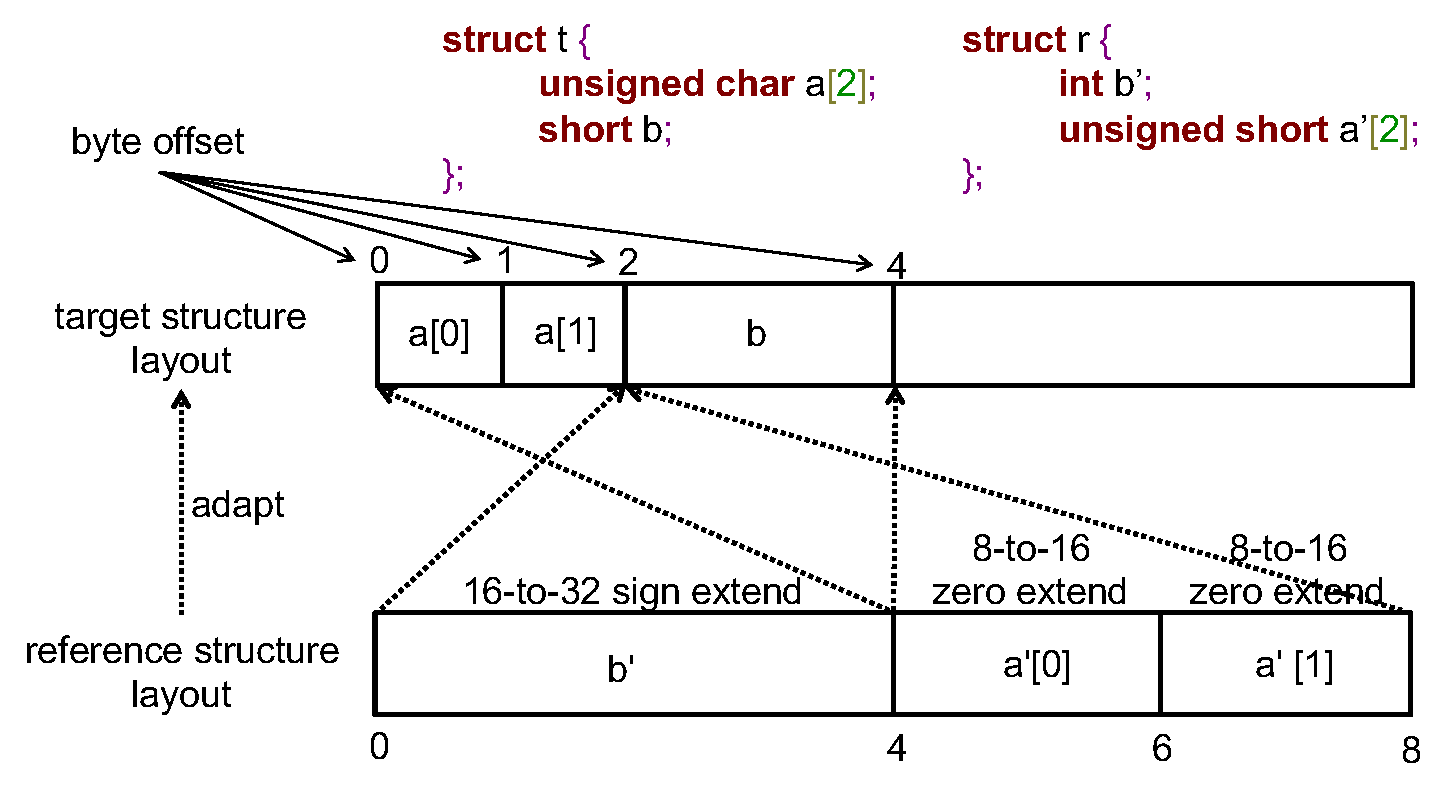
\includegraphics[width=\widthfactor\columnwidth]{chapters/adapter_synthesis/figures/memsub_pdf6}
\end{figure}  
\subsubsection{Return Value Substitution}
The argument substitution families described above can also be applied on return values.
%
An example of different return values having the same semantic meaning is the return value of the C library function \textit{isalpha} as shown in Listing \ref{lst:isalpha}.
%
The wrapper function \textit{adapted\_isalpha} in Listing~\ref{lst:isalpha} performs
return value substitution.
%
%As per the C library specification, the functions \textit{isalpha}, \textit{isalnum} must return a non-zero value if their argument is a digit, a alphabet, or a alphanumeric character respectively, and return zero otherwise.
%
%While any non-zero return value for these two functions has the same semantic meaning, when these predicates are satisfied, the eglibc library implementation~(the system C library commonly available on Ubuntu 14.04) of these two functions returns non-zero values from these two functions that are different from those returned by the musl, a newer implementation of the C library specification.
%
%This example provides motivation for this family of adapters because changing a nonzero return value of such predicate functions to 1 harmonizes the difference between return values of the same isalpha predicate. \\ %can create functional equivalence as shown in Listing \ref{lst:return_adapter}. 
%
%\lstinputlisting[caption={Return value substitution adapter example}, label={lst:return_adapter}, style=nonumbers]{code_samples/return-adapter.c}
%
%This is shown in Listing \ref{lst:arithmetic_bit_synthesis}. 
%\lstinputlisting[caption={Arithmetic adapter example}, label={lst:arithmetic_bit_synthesis}, style=nonumbers]{code_samples/arithmetic-bit-synthesis.c}
%    \textbf{Character Set Translation adapter:}
%    %\subsubsection{Character Set Translation adapter}
%    The \textit{chartrans} rule in Grammar \ref{grammars} translates each character according to some fixed mapping.
%    The \textit{tr} function provides character set translations similar to the \texttt{tr} Unix utility (without squeezing or deleting characters) in string arguments.
%    The \textit{LIST1} and \textit{LIST2} terminals in the \textit{chartrans} rule specify the source-to-destination mapping.
%    e.g. the first character in \textit{LIST1} is translated to the first character in \textit{LIST2}.
%    \todo{example ?}
%Listing \ref{lst:chartrans_adapter} shows an example application of this adapter grammar. 
%While both \textit{$f_1$} and \textit{$f_2$} check whether a the input string is a palindrome, \textit{$f_1$} expects the string to be newline-terminated and \textit{$f_2$} expects the string string to be null-terminated. 
%The adapter between \textit{$f_1$} and \textit{$f_2$} translates every instance of the newline character to the null character.

% \lstinputlisting[caption={Character set translation adapter example}, label={lst:chartrans_adapter}, style=nonumbers]{code_samples/chartrans-adapter.c}

\subsection{Example}
%
\begin{figure}
\lstinputlisting[caption={Two implementations of similar adaptable functionality}, label={lst:example}, style=nonumbers]{chapters/adapter_synthesis/code_samples/example.c}
\end{figure}
%
To illustrate our approach, we walk through a representative run of our adapter synthesis algorithm using a pair of target and reference functions that implement similar functionality.
%
Both the target and reference functions are shown in Listing~\ref{lst:example}. 
%
Here we will focus only on synthesis of the input adapter, although the general algorithm also produces an adapter that adapts the output of the reference function. 
%
A correct input adapter should set the first argument of \texttt{reference} to the integer argument $y$ of \texttt{target} and set the second argument to the constant 1 to adaptably substitute the \texttt{y \% 2} operation in \texttt{target}.
%
It should also set both the third and fourth arguments of \texttt{reference} to the first argument of \texttt{target} to adaptably substitute the \texttt{x << 1} operation in \texttt{target}. 
%
We write this adapter as $\mathcal{A}(x,y) = (y, 1, x, x)$.

\textbf{Step 0:} 
Adapter synthesis begins with an empty counterexample list and a default adapter that maps every argument to the constant 0 (i.e. $\mathcal{A}(x,y) = (0,0,0,0)$). During counterexample generation (\texttt{CheckAdapter} in Figure~\ref{fig:adapter_synthesis}), we use symbolic execution to search for an inputs $x,y$ such that the output of \texttt{target(x,y)} is not equivalent to the output of \texttt{reference(}$\mathcal{A}(x,y)$\texttt{)} = \texttt{reference(0,0,0,0)}. From \texttt{CheckAdapter}, we learn that $x = 1, y = 0$ is one such counterexample.
 
\textbf{Step 1:} Next, during adapter search (\texttt{SynthesizeAdapter} in Figure~\ref{fig:adapter_synthesis}), we use symbolic execution to search for a new adapter $\mathcal{A}$ that will make \texttt{target(x)} equivalent to \texttt{reference(}$\mathcal{A}(x,y)$\texttt{)} for all inputs $x,y$ in the list [(1,0)]. From \texttt{SynthesizeAdapter}, we learn that $\mathcal{A}(x,y) = (y,y,x,x)$ is a suitable adapter, and this becomes our new current adapter.

\textbf{Step 2:} We use \texttt{CheckAdapter} to search for a counterexample to the current adapter, $\mathcal{A}(x,y) = (y,y,x,x)$. We find that $x = 0, y = 3$ is a counterexample. 

\textbf{Step 3:} Next, we use \texttt{SynthesizeAdapter} to search for
an adapter $\mathcal{A}$ for which the output of \texttt{target(x)} will
be equivalent to the output of
\texttt{reference(}$\mathcal{A}(x,y)$\texttt{)} for both pairs of
inputs, $x = 1, y = 0$ and $x = 0, y = 3$. \texttt{SynthesizeAdapter} identifies $\mathcal{A}(x) = (y,1,x,x)$ as a suitable adapter.

\textbf{Step 4:}
At the beginning of this step, the current adapter is $\mathcal{A}(x,y) = (y,1,x,x)$. As before, we use \texttt{CheckAdapter} to search for a counterexample to the current adapter. We find that \texttt{CheckAdapter} fails to find a counterexample for the current adapter, indicating that the current adapter is correct for all explored paths. Therefore, adapter synthesis terminates with the final adapter $\mathcal{A}(x) = (y, 1, x, x)$.
%Alternatively, adapter synthesis could have terminated with the decision that the target function is not substitutable by the reference function with any allowed adapter.
%In our evaluations, adapter synthesis may also terminate with a timeout, indicating the total runtime has exceeded a predefined threshold.

\subsection{Extensibility}

The adapter synthesis algorithm presented in this section is not tied to a source programming language or adapter family.
In our implementation (Section~\ref{sec:implementation}) we target
binary x86 and ARM code, and we use adapters that allow for common
argument structure changes found in binaries compiled from C and C++ code.
Because we work at the binary level, we are also not restricted to working at the level of target functions as described so far.
In Section~\ref{subsec:eval_general}, instead of target functions, we consider target ``code fragments.''
We define a code fragment to be a sequence of instructions consisting of at least one instruction. 
Inputs to code fragments are the general-purpose registers available on the architecture of the code fragment and outputs are registers written to within the code fragment.
%
We could similarly allow reference functions to be more general code regions.



\section{Implementation}\label{sec:implementation}

%\subsection{Tools}
We implement adapter synthesis for Linux/x86-64 binaries using
the symbolic execution tool FuzzBALL~\cite{fuzzball}, which is freely available~\cite{fuzzball-github}.
%Symbolic execution determines what inputs to a program will cause certain behaviors.
%The idea is to execute the program of interest with some concrete values replaced by symbolic variables, and to find satisfying assignments to those symbolic variables that cause the desired execution path to be explored.
FuzzBALL allows us to explore execution paths through the target and
adapted reference functions to (1) find counterexamples that invalidate previous candidate adapters and (2) find candidate adapters that create behavioral equivalence for the current set of tests. 
%
As FuzzBALL symbolically executes a program, it constructs and maintains Vine IR expressions using the BitBlaze~\cite{bitblaze-url} Vine library~\cite{bitblaze-vine} and interfaces with the STP~\cite{stp} decision procedure to solve path conditions.
%
We also evaluate adapter synthesis by replacing the symbolic execution-based implementation of adapter search with a concrete implementation that searches the adapter space in a random order.
%
\subsection{Test Harness}
%
To compare code for equivalence we use a test harness similar to the one used by Ramos et al.~\cite{Ramos:2011:PLE:2032305.2032360} to compare C functions for direct equivalence using symbolic execution.
%
The test harness exercises every execution path that passes first through the function, and then through the adapted reference function.
%
As FuzzBALL executes a path through the function, it maintains a path condition that reflects the branches that were taken.
%
As execution proceeds through the adapted reference function on an execution path, FuzzBALL will only take branches that do not contradict the path condition.
%
Thus, symbolic execution through the target and reference functions consistently satisfies the same path condition over the input.
%
Listing \ref{lst:test_harness} provides a representative test harness.
%
If the target is a code fragment instead of a function, its inputs $x_1$, ..., $x_n$ need to be written into the first $n$ general purpose registers available on the architecture.
%
Since the target code fragment may write into the stack pointer register ({\tt sp} on ARM), the value of the stack pointer also needs to be saved before executing the target code fragment and restored after the target code fragment has finished execution.
%
On line 2 the test harness executes
\texttt{TARGET} with inputs $x_1$, ..., $x_n$ and captures its output in {\tt r1}.
%
If the target is a function, its outputs are its return value and values
written to memory.
%
If the target is a code fragment, its output needs to be determined in a preprocessing phase.
%
One heuristic for choosing a code fragment\rq s output is to choose the last register that was written into by the code fragment.
%
On line 6, the test harness calls the adapted reference function \texttt{REF} with
inputs $y_1$, ..., $y_m$, which are derived from $x_1$, ..., $x_n$ using
an adapter \texttt{A}.
%
After executing {\tt REF}, the test harness adapts {\tt REF}\rq s return value using the return adapter {\tt R} and saves the adapted return value in {\tt r2}.
%
On line 7 the test harness branches on whether the results of the calls to the target and adapted reference code match.
%
\lstinputlisting[caption={Test harness}, label={lst:test_harness}]{chapters/adapter_synthesis/code_samples/compare.c}
%

We use the same test harness for both counterexample search~(called
		\texttt{CheckAdapter} in Figure~\ref{fig:adapter_synthesis}) and
adapter search~(called \texttt{SynthesizeAdapter} in
		Figure~\ref{fig:adapter_synthesis}). 
%
During counterexample search, the inputs $x_1$, ..., $x_n$ are marked as
symbolic and the adapters {\tt A} and {\tt R} are concrete.
%
FuzzBALL first executes the function using the symbolic $x_1$, ..., $x_n$.
%
It then creates reference function arguments $y_1$, ..., $y_n$ using the
concrete adapter \texttt{A} and executes the reference function.
%
During adapter search, for each set of test inputs $x_1$, ..., $x_n$, FuzzBALL first executes the function concretely.
%
The adapter \texttt{A} is then marked as symbolic, and FuzzBALL then applies symbolic adapter formulas (described in \ref{sec:adapter_formulae}) to the concrete test inputs and passes these symbolic formulas as the adapted reference function arguments $y_1$, ..., $y_n$.
%
During counterexample search we are interested in paths that execute the ``Mismatch'' side, and during adapter search we are interested in paths that execute the ``Match'' side of the branch on line 7 of Listing \ref{lst:test_harness}.
%
For simplicity, Listing \ref{lst:test_harness} shows only the return values $r_1$ and $r_2$ as being used for equivalence checking.
%
%However, during symbolic execution we extend this test harness to do equivalence checking of other state information, including memory and system calls, when comparing the target and adapted reference code executions.
%
\subsection{Adapters as Symbolic Formulae}
\label{sec:adapter_formulae}
%
% \lstinputlisting[label=lst:typeconv_adapter_formula,label={lst:typeconv_adapter_formula},caption={Vine IR formula for one type conversion operation and argument substitution}]{code_samples/typeconv_adapter_formula.c}
% 
We represent adapter families in FuzzBALL using Vine IR expressions involving symbolic variables.
%
For example, an adapter from the argument substitution family for the adapted
reference function argument $y_i$ is represented by a Vine IR expression that indicates whether $y_i$ should be replaced by a constant value (and if so, what constant value) or an argument from the target function (and if so, which argument).
%
This symbolic expression uses two symbolic variables, \textit{y\_i\_type} and \textit{y\_i\_val}.
%
We show an example of an adapter from the argument substitution family represented as a symbolic formula in Vine IR in Listing \ref{lst:simple_adapter_formula}.
%
This listing assumes the target function takes three arguments, \textit{x1}, \textit{x2}, \textit{x3}.
%
This adapter formula substitutes the adapted reference function argument \textit{y1} with either a constant or with one of the three target function arguments.
%
A value of 1 in \textit{y\_1\_type} indicates \textit{y1} is to be substituted by the constant value given by \textit{y\_1\_val}.
%
If \textit{y\_1\_type} is set to a value other than 1, \textit{y1} is to be substituted by the target function argument at the position present in \textit{y\_1\_val}.
%
We constrain the range of values \textit{y\_1\_val} can take by adding side conditions. 
%
In the example shown in Listing \ref{lst:simple_adapter_formula}, when \textit{y\_1\_type} equals a value other than 1, \textit{y\_1\_val} can only equal 0, 1, or 2 since the target function takes 3 arguments.
%
% Symbolic formulae for argument substitution can be extended naturally to more complex adapter families by adding additional symbolic variables.
% %
% For example, consider the Vine IR formula shown in Listing~\ref{lst:typeconv_adapter_formula} which extends the formula in Listing~\ref{lst:simple_adapter_formula} to allow sign extension from the low 16 bits of a value.
% %
% Listing \ref{lst:typeconv_adapter_formula} begins in the same way as Listing \ref{lst:simple_adapter_formula} on line 1.
% %
% But, this time, if \textit{y\_1\_type} is 0, it performs argument substitution based on the value in \textit{y\_1\_val} on lines 3, 4.
% %
% If \textit{y\_1\_type} is any value other than 0, it performs sign extension of the low 16 bits in a value.
% %
% This value is chosen based on the position set in \textit{y\_1\_val} on lines 8, 9.
% %
% Notice lines 8, 9 are the same as lines 3, 4, which means the value, whose low 16 bits are sign-extended, is chosen in exactly the same way as argument substitution.
%
%
\lstinputlisting[caption={Argument Substitution adapter}, label={lst:simple_adapter_formula}, style=nonumbers]{chapters/adapter_synthesis/code_samples/simple_adapter_formula.c}
%
During adapter search, Vine IR representations of adapted reference function arguments are placed into argument registers of the reference function before it begins execution, and placed into the return value register when the reference function returns to the test harness.
%
When synthesizing memory substitution adapters, Vine IR formulas allowing memory substitutions are written into memory pointed to by reference function arguments.
%
We use the registers \%rdi, \%rsi, \%rdx, \%rcx, \%r8, and \%r9 for function arguments and the register \%rax for function return value, as specified by the x86-64 ABI calling convention~\cite{x64-abi}.
%
We do not currently support synthesizing adapters between functions that use arguments passed on the stack, use variable number of arguments, or specify return values in registers other than \%rax.
%
%Our adapter synthesis tool does not support floating point type arguments, but it can be easily extended to allow symbolic formulae on floating point inputs.
%
%While we limit our implementation to synthesize adapters at the function interface level only up to six function arguments, we find a significant portion of the functions in the glibc library are still available for adapter synthesis. 
%
%For synthesizing memory substitution adapters, we write symbolic formulas which allow memory substitution into all addresses used by the target function, up to limited bytes.
%
%Using a smaller limit allows the symbolic formulas to be small and easy to solve but prevents larger structures from being adapted.
%We do not support synthesizing adapters when the function interface of either the target or adapted reference function uses a value of floating point type.
%
\subsection{Equivalence checking of side-effects}
\label{sec:eqchk-syscall}
We allow target and reference code to make system calls and have side-effects on memory.
%
We record the side-effects of executing the target and adapted reference functions and compare them for equivalence on every execution path.
%
For equivalence checking of side-effects via system calls, we check the sequence of system calls and their arguments, made by both functions, for equality.
%
For equivalence checking of side-effects on concretely-addressed memory, we record write operations through both functions and compare the pairs of (address, value) for equivalence.
%
For equivalence checking of side-effects on memory addressed by symbolic values, we use a FuzzBALL feature called \textit{symbolic regions}. 
%
Symbolic address expressions encountered during adapted reference function execution are checked for equivalence with those seen during target function execution and mapped to the same symbolic region, if equivalent.
%
%We describe our implementation of equivalence checking on side-effects in more detail in Section \ref{subsec:eqchk-se} in the Appendix. 

%\todo[inline]{Write subsections on equivalence checking for concretely-addressed memory and symbolic regions}


\section{Evaluation}\label{sec:evaluation}
%
In this section, we evaluate the performance of adapter synthesis and
present its applications using case studies.
%
In Section~\ref{subsec:case-study-security}, we present an example of finding
adaptable substitutability modulo a bug---enabling programmers to more easily replace buggy
components of their code.
%
In Section~\ref{subsec:rc4-experiment}, we show how our technique can
enable programmers to switch between different libraries with the same
functionality.
%
In Section~\ref{subsec:c-library-evaluation}, we show that adapter
synthesis can find adapters even within a library.
%
In Section~\ref{subsec:conc-search}, we compare symbolic execution-based adapter search
with concrete enumeration-based adapter search.
%
Finally, in Section~\ref{subsec:eval_general}, we show how our technique can be used for
reverse engineering.
\subsection{Case Study: Security}\label{subsec:case-study-security}
%
\lstinputlisting[caption={Two implementations for mapping ordered keys, negative or positive, to values using a C array},
label={lst:lookup}]{chapters/adapter_synthesis/code_samples/lookup.c}
%
%Data structures that map keys to their corresponding values are commonly found in modern programming languages~\cite{hashtbl-ocaml},~\cite{map-cpp}. 
%
%Support for such data structures is not part of the C language standard.
%
%Arrays in C provide a convenient and fast way for mapping a previously known number of integer keys to values.
%
%Implementation of data compression algorithms and signal processing implementations require constant-time lookup for negative and positive powers of values.
%
%In such situations, an array in C can be the perfect solution.
%
Consider a table implementing a function of a signed input.
%
For example, keys ranging from -127 to 127 can be mapped to a 255-element array.
%
Any key \textit{k} will then be mapped to the element at position \textit{k}+127 in this array.
%
We present two implementations of such lookup functions in Listing~\ref{lst:lookup}.
%
Both functions, \textit{lookup1} and \textit{lookup2}, assume keys ranging from $-$\textit{len}/2 to +\textit{len}/2 are mapped in the \textit{table} parameter with \textit{lookup1} being specific to tables of length 255.
%
However, \textit{lookup1} contains a bug caused by undefined behavior.
%
The return value of \textit{abs} for the most negative 32-bit integer~(-2147483648)~is not defined~\cite{gnu-abs}.
%
Given the most negative 32-bit integer, the eglibc-2.19 implementation of \textit{abs} returns that same 32-bit integer.
%
This causes the check on line 2 of Listing~\ref{lst:lookup} to not be satisfied, allowing execution to continue to line 5 and causing an out-of-bounds memory access.
%
\textit{lookup2} in Listing~\ref{lst:lookup} is a different implementation of an array-based lookup with a different interface than \textit{lookup1}.
%
Checking whether the key is in range is done differently in \textit{lookup2}, causing it to not have the memory access bug present in \textit{lookup1}.
%
For this reason, users of \textit{lookup1} may find it desirable to substitute the use of \textit{lookup1} with \textit{lookup2}.
%
Adapter synthesis can perform such a substitution by adapting \textit{lookup2} to \textit{lookup1} while simultaneously not adapting the out-of-bounds memory access in \textit{lookup1}.
%
Our adapter synthesis implementation synthesizes the correct argument substitution adapter in the \textit{lookup1} $\leftarrow$ \textit{lookup2} direction in about 8 minutes.
%
Synthesis of the correct adapter is slowed down by the presence of the \textit{table} pointer in the interfaces of \textit{lookup1} and \textit{lookup2}.
%
The adapter is shown on lines 15-18 of Listing~\ref{lst:lookup}.
%
This case study shows adapter synthesis can replace a buggy function
with its bug-free variant by doing adaptation modulo a bug.
%
\subsection{Case Study: Library Replacement}\label{subsec:rc4-experiment}
%
To show that adapter synthesis can be applied to replace functionality
from one library with that from another library, we adapt functions implementing RC4 functionality in mbedTLS and OpenSSL.
\noindent
\subsubsection{RC4 context initialization} The RC4 algorithm uses a
variable length input key to initialize a table with 256 entries within
the context argument.
%
Both cryptography libraries in our example, mbedTLS and OpenSSL, have their own implementation of this initialization routine.
%
Both initialization function signatures are shown in Figure \ref{fig:rc4setup_adapter}.
%
\begin{figure}[]
	\centering
	\caption{Argument substitution adapter to make \textit{RC4\_set\_key} adaptably equivalent to \textit{mbedtls\_arc4\_setup}}
	\label{fig:rc4setup_adapter}
	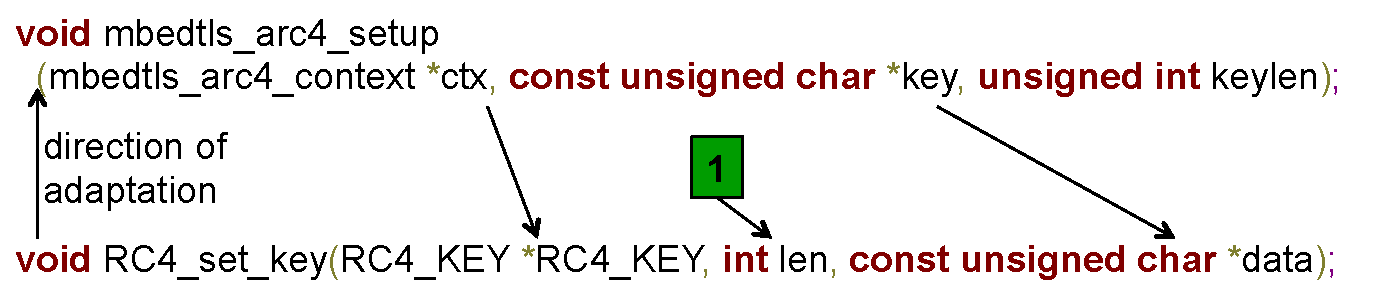
\includegraphics[width=\widthfactor\columnwidth]{chapters/adapter_synthesis/figures/rc4setup_adapter}
\end{figure}
%
Executing each of these initialization routines requires 256 rounds of
mixing bytes from the key string into the context.
%
%Each round requires two load and two store operations into an array with 256 entries.
%
The two initialization routines require the key length and key string arguments at different positions, and use different RC4 context structures (\textit{RC4\_KEY} in OpenSSL, \textit{mbedtls\_arc4\_context} in mbedTLS).
%
The RC4 context arguments contain three fields as shown in Figure \ref{fig:rc4_struct_adapter}.
%
\begin{figure}[]
	\centering
	\caption{Memory substitution adapter to make \textit{RC4\_KEY} adaptably equivalent to \textit{mbedtls\_arc4\_context}}
	\label{fig:rc4_struct_adapter}
	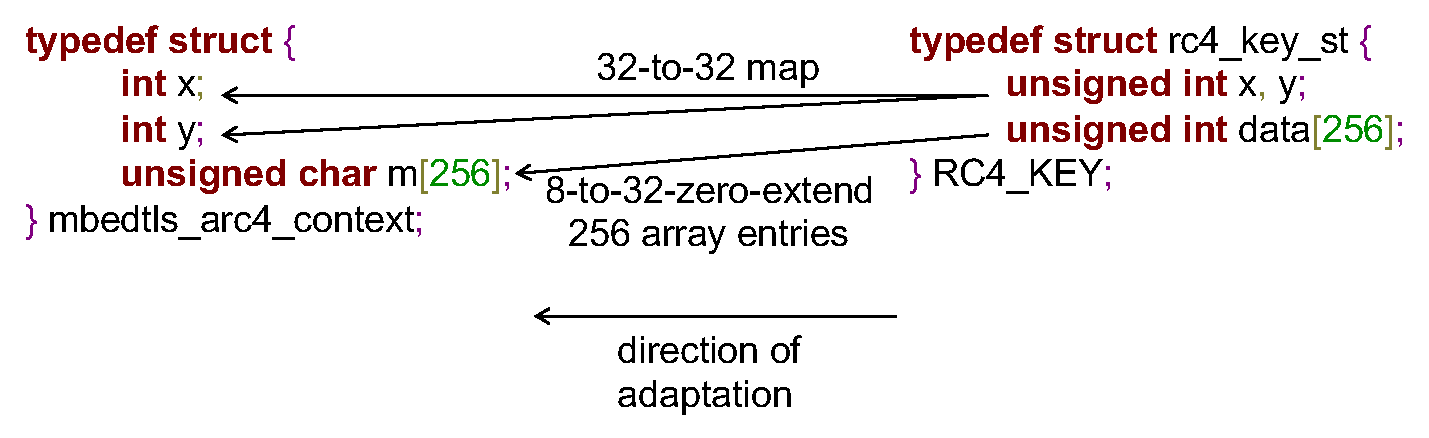
\includegraphics[width=\widthfactor\columnwidth]{chapters/adapter_synthesis/figures/rc4_struct_adapter}
\end{figure}
%
The first two 4-byte fields are used to index into the third field, which is an array with 256 entries.
%
Each entry in the array is 4 bytes wide in OpenSSL and 1 byte wide in mbedTLS.
%
The correct adapter that adapts the OpenSSL context to the mbedTLS
context~(mbedTLS $\leftarrow$ OpenSSL) performs two mapping operations:
(1) it maps the first two mbedTLS context\rq s fields directly to the
first two OpenSSL context\rq s fields and (2) it zero extends each 1 byte
entry in the third field of the mbedTLS context to the corresponding 4
byte entry in the third field of the OpenSSL context.
%
The correct adapter for making the \textit{RC4\_KEY} structure adaptably
equivalent to the \textit{mbedtls\_arc4\_context} structure is shown in Figure \ref{fig:rc4_struct_adapter}.
%
The correct adapter in the reverse direction~(OpenSSL $\leftarrow$ mbedTLS) changes the second mapping operation to map the least significant byte of each 4 byte entry in the third field to the 1 byte entry in its corresponding position.

Performing this adaptation with \textit{mbedtls\_arc4\_setup} and
\textit{RC4\_set\_key}~(the RC4 context initialization functions in
mbedTLS and OpenSSL respectively) requires adaptation of side-effects on memory
because mixing of the key string into the context is the only output of these functions.
%
Since a memory substitution structure can be used both as input and as output, we have to perform the memory substitution adaptation at least twice.
%
First, the reference function may use the memory substitution structure as input.
Hence, we need to adapt the initial byte values of the memory substitution structure to obtain the initial byte values to be used for the reference function.
%
Second, before running the reference function, the target function could have written to the memory substitution structure.
Hence, we need to adapt side-effects of the target function on the memory substitution structure in order to compare them with corresponding side-effects on memory from the reference function.
%
The most general memory substitution adapter synthesis allows arbitrary
numbers of 1, 2, 4, or 8 byte entries in each field of the
264~($2 \times 4 + 256 \times 1$) byte mbedTLS context and 1032~($2 \times 4+256 \times 4$) byte OpenSSL
context.
%
But this makes the search space of memory mappings very large.
%
We instead only explored adapters where the number of entries in each array was a power of 2.
%
While this reduction is useful in practice, it still gives us a search space of about 4.7 million possible memory substitutions in both directions of adaptation.

Finally, memory substitution must be combined with argument substitution to synthesize adapters between \textit{mbedtls\_arc4\_setup} and \textit{RC4\_set\_key}.
%
This combination of argument substitution and memory substitution adapter families creates a search space of 5.593 billion adapters.
%Vaibhav: I got this number of adapters by multiplying 4.7 million memory substitution adapters with the argument substitution number for f1nargs = 3, f2nargs = 3, const_lb = 1, const_ub = 1, return value substitution adapters = 8*f2nargs + 9 + (const_ub - const_lb + 1) + 1. We ran this adapter synthesis with the full return value substitution adapter. The exact calculation code is on mccarran:/export/scratch/vaibhav/tests/calc_num_adaptors.c
%
Our adapter synthesis tool figures out the correct argument,
memory, and return value substitutions.
%
It finds adaptable equivalence in both directions of adaptation by checking equivalence between side-effects on the structure objects~(\textit{ctx} for \textit{mbedtls\_arc4\_setup}, \textit{RC4\_KEY} for \textit{RC4\_set\_key}).
%
The correct adapter for adaptably substituting the
\textit{mbedtls\_arc4\_setup} function with the \textit{RC4\_set\_key}
function is shown in
Figure~\ref{fig:rc4setup_adapter}.
%
To setup adapter synthesis between these two function pairs (we synthesized adapters in both directions), we used a symbolic key string of length 1, and hence the synthesis tool correctly sets the key length argument to 1.
%
While we acknowledge that using an input string of length 1 is too small to be useful, we expect the adapter to be correct on strings of length greater than 1 in practice.
%
We also plan to integrate techniques such as path merging~\cite{KuznetsovKBC2012,AvgerinosRCB2014} to increase the bounds of inputs used in adapter synthesis.
%
While we used an input memory substitution size of 1032 symbolic bytes for memory substitution, both \textit{mbedtls\_arc4\_setup} and \textit{RC4\_set\_key} initialize this memory with concrete values in their implementation, thereby causing this adaptation to start with a much smaller symbolic state consisting of a single symbolic input byte.

We present the time taken to synthesize adapters for RC4 setup function
pairs in Table~\ref{table:rc4-adapter-synthesis-days}.
%
The execution time shown in Table~\ref{table:rc4-adapter-synthesis-days}
for concrete enumeration-based adapter search is the average execution time
taken for adapter synthesis over 10 correctly synthesized adapters for
adapting RC4 setup functions.
%
We performed adapter synthesis using concrete enumeration-based adapter
search 10 times because concrete enumeration-based adapter search
traverses the adapter space in a random order.
%
Using the execution times shown in Table~\ref{table:rc4-adapter-synthesis-days}
and the observation that our adapter synthesis never used more than 1 CPU core
and 4 GB of RAM, we estimated~\cite{amazon-ec2-pricing} the cost of
this computation on a Amazon EC2 instance~(t2-medium).
%
Table~\ref{table:rc4-adapter-synthesis-cost} shows these estimated costs.
%
These costs suggest that automated
adapter search is likely competitive with paying a human programmer to find
and verify the correctness of an adapter at the binary level.
%
The time required for adapter synthesis can be
further reduced by parallelizing the adapter search in concrete
enumeration and reusing the state of adapter search in FuzzBALL-based
adapter search.
%
We discuss this further in Section~\ref{sec:future_work}.
%
%Thus, we combined the memory substitution adapter with the argument substitution adapter family to synthesize adaptable equivalence between the RC4 setup functions.
%
\noindent
%
\input{chapters/adapter_synthesis/tables/rc4-adapter-synthesis-days}
\input{chapters/adapter_synthesis/tables/rc4-adapter-synthesis-cost}
%
\subsubsection{RC4 encryption} The RC4 encryption functions in mbedTLS and
OpenSSL take 4 arguments each, three of which are pointers to the RC4
context, the input key string, and the output string, as shown in
Figure~\ref{fig:rc4-encrypt-mo}.
%
\begin{figure}[]
	\centering
	\caption{Adapter performing argument and memory substitution to make
	\textit{mbedtls\_crypt} in the mbedTLS library adaptably substitutable
	by \textit{RC4} in OpenSSL}
	\label{fig:rc4-encrypt-mo}
	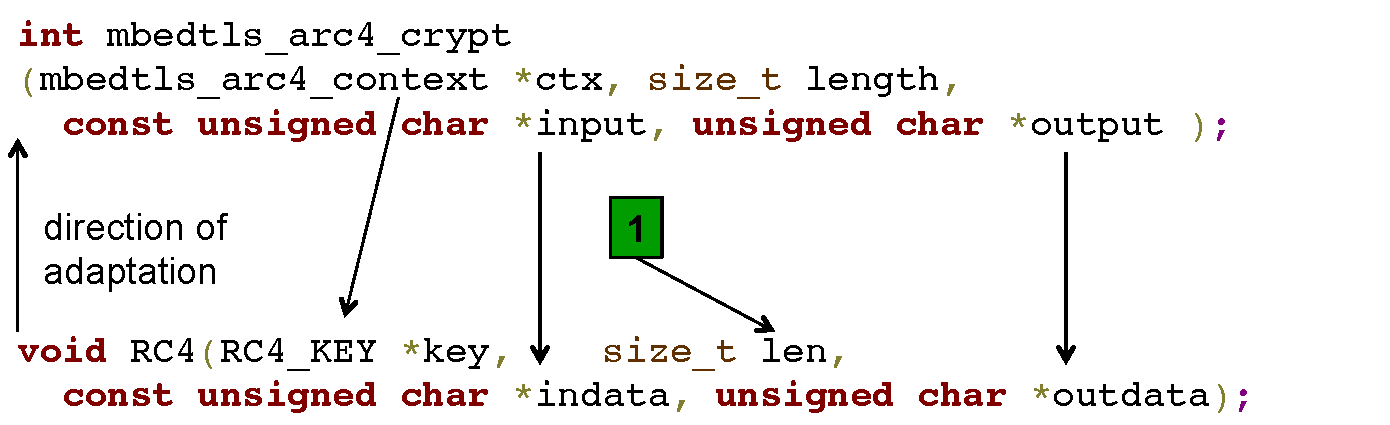
\includegraphics[width=\widthfactor\columnwidth]{chapters/adapter_synthesis/figures/rc4-encrypt-mo}
\end{figure}
%
These functions use the RC4 context as input, causing the initial symbolic state to consist of 1032 symbolic bytes for memory substitution and one symbolic byte for the input string.
%
These functions both read from and write to the RC4 context, making
two memory substitution adaptations necessary.
%
These functions also encrypt every byte of the input string using a loop where the length of the input string is given as a parameter to the function.
%
Since all arguments to the reference function are symbolic, using a symbolic formula for the length of the input string can easily cause the loop bound to be very large, especially if the symbolic formula for the length allows the possibility of the length being equal to one of the pointer arguments to the reference function.
%
To avoid the encryption loop in the reference function from executing too many times, we restricted every instruction in the reference function to be executed at most twice.
%
Finally, because these functions write to an output string, it is
necessary for us to have memory side-effects equivalence checking to
capture outputs that are not part of the return value.

The adapter search space in this case consists of $1.792 \times 10^{12}$ adapters.
%Vaibhav: I got this number by by multiplying 4.7 million memory substitution adapters with the argument substitution number for f1nargs = 4, f2nargs = 4, const_lb = 0, const_ub = 5, return value substitution adapters = 8*f2nargs + 9 + (const_ub - const_lb + 1) + 1. We ran this adapter synthesis with the full return value substitution adapter. The exact calculation code is on mccarran:/export/scratch/vaibhav/tests/calc_num_adaptors.c 
%
The correct adapter for making the \textit{RC4} method adaptably
equivalent to \textit{mbedtls\_arc4\_crypt} is shown in Figure
\ref{fig:rc4-encrypt-mo}.
%
Our adapter synthesis tool finds the correct argument and memory
substitution adapters in both directions of adaptation.
%
Tables~\ref{table:rc4-adapter-synthesis-days},~\ref{table:rc4-adapter-synthesis-cost}
show the time taken for and estimated cost of adapter synthesis between
the RC4 encryption functions in OpenSSL and mbedTLS.
%
Once again, the execution time shown in Table~\ref{table:rc4-adapter-synthesis-days}
for concrete enumeration-based adapter search is the average execution time
taken for adapter synthesis over 10 correctly synthesized adapters.
%
We verified the correctness of our adapted context structures by using self-tests present in mbedTLS and OpenSSL.
%
%Given the design of the RC4 encryption algorithm, we do not expect the correctness of our adapters to change for longer input strings.
%
\noindent
\subsubsection{On improving memory substitution performance} On
combining the memory substitution adapter family with argument and
return value substitution, our adapter synthesis tool encountered a
significant slowdown with both RC4 context initialization and encryption.
%
This can be attributed in part to the encoding of memory substitutions in our tool.
%
We enumerate all possibilities of memory substitutions into the formula of every byte in the memory substitution structure, causing the symbolic formulas to be very large.
%
We plan to encode the memory substitution adapter more efficiently in the future to make better use of existing solvers.
%
Another significant cause of the slowdown, in the case of RC4 context initialization, is the slow symbolic execution of 256 rounds of key mixing, once in the target and once in the reference function, because of two symbolic loads and two symbolic stores to memory on every round of key mixing.
%
We plan to integrate loop summarization~(for example, as described by
Godefroid et al.~\cite{godefroid2011}), and use the theory of arrays for symbolically-indexed memory accesses to speed up this symbolic execution in the future.
%
In the case of RC4 encryption, since we have to adapt the memory substitution structures twice (once for input and once for output) we have to present large formulas to the solver at least twice on every execution path with each query taking a few seconds.
%
This large symbolic state is the cause of significant slowdown during RC4 encryption adapter synthesis.
%
We plan to explore concretization heuristics of symbolic bytes in the future to reduce the number of solver invocations made during RC4 encryption adapter synthesis.
%
\noindent
\subsubsection{RC4 adapter verification using nmap} We verified the
correctness of our RC4 memory substitution adapter using nmap with the setup shown in Figure \ref{fig:nmap_struct_adapter}.
%
\begin{figure}[]
	\centering
	\caption{nmap using RC4 encryption in mbedTLS instead of OpenSSL}
	\label{fig:nmap_struct_adapter}
	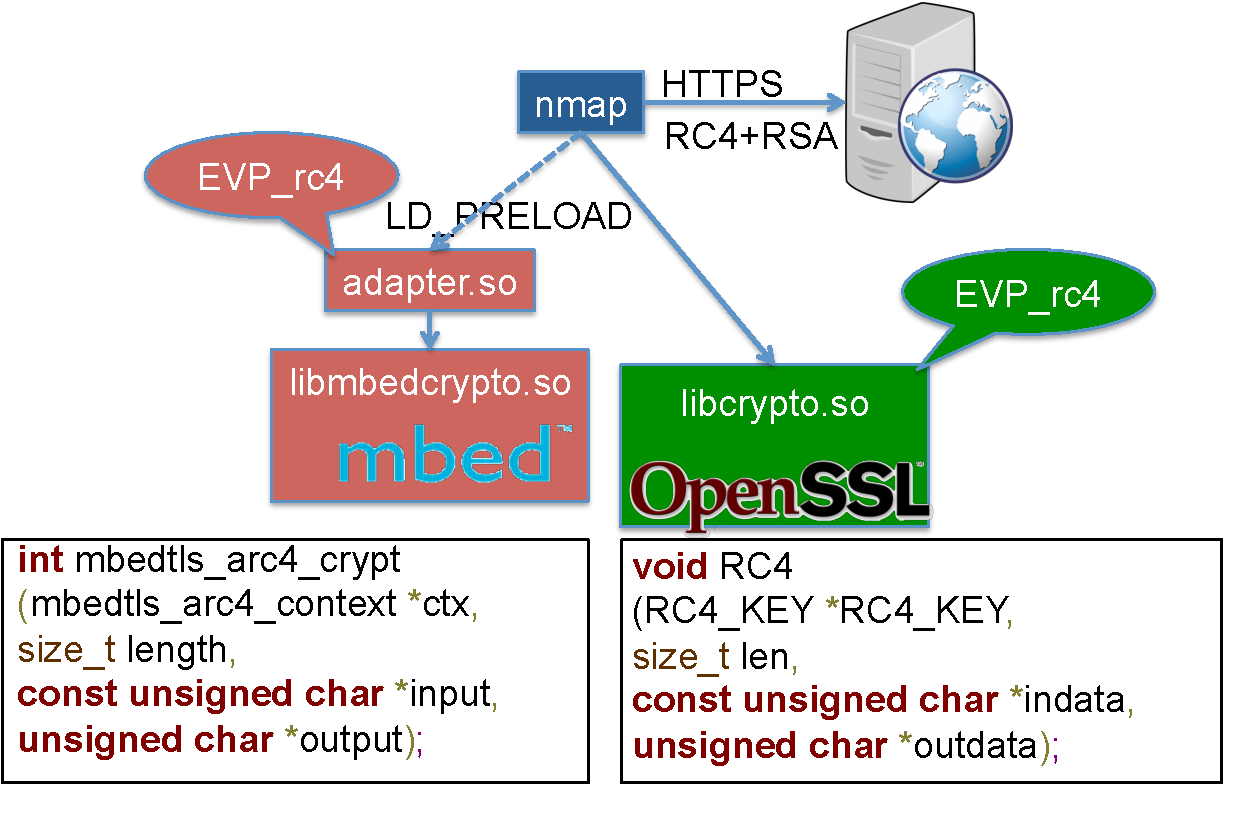
\includegraphics[width=\widthfactor\columnwidth]{chapters/adapter_synthesis/figures/nmap_struct_adapter}
\end{figure}
%
We created adapted versions of the OpenSSL RC4 setup and encryption
functions that internally use the mbedTLS context adapted to the OpenSSL
context.
%
On a 64-bit virtual machine running Ubuntu 14.04, we compiled the adapted setup and encryption functions into a shared library and setup a local webserver, which communicated over port 443 using the \textit{RC4+RSA} cipher.
%
We used the stock nmap binary to scan our localhost and injected our specially created shared library using the \textit{LD\_PRELOAD} environment variable.
%
The preloading caused the RC4 functions in our shared library to be executed instead of the ones inside OpenSSL.
%
The output of nmap, run with preloading our specially created shared library which used the OpenSSL $\leftarrow$ mbedTLS structure adapter, was the same as the output of nmap when using the system OpenSSL library.
%
\subsection{Intra-library Adapter Synthesis}
\label{subsec:c-library-evaluation}
%
The previous section showed an application of adapter synthesis where the target and reference functions came from
independently-developed implementations.
%
But, adapter synthesis can also be useful in cases where the target and reference functions were developed within the same
library.
%
Synthesizing adapters between binary functions in the same library can expose important relations between adaptably
substitutable functions that may not be known to users of the library.
%
It can show relations between functions, by, for example showing that one function can be adaptably
implemented in terms of another.
%
Verifying such relations between functions from their binary implementation can provide the users of the library a
more detailed picture of the function\rq s behavior.
%
In libraries with a large interface, such as the Ubuntu 14.04 system C library, where it can be challenging to manually identify
adaptability relations between functions, performing automated intra-library adapter synthesis can be particularly
useful.
%
\subsubsection{Setup}
%
We evaluated our adapter synthesis tool on the system C library available on Ubuntu 14.04~(eglibc 2.19).
%
The C library uses a significant amount of inlined assembly, for instance, the \textit{ffs}, \textit{ffsl}, \textit{ffsll} functions, which
motivates automated adapter synthesis at the binary level.
%
We enumerated 1316 exported functions in the library in the order they
appear, which caused functions that are defined in the same source files
to appear close to each other.
%
Considering every function in this list as the target function, we chose five functions that appear above and below it as 10 potential reference functions.
%
These steps gave us a list of 13130~($10\times 1316 - 2 \times \sum_{i=1}^5 i$) pairs of target and reference functions.
%since the first five and the last five target functions 
%had less than five potential semantically-equivalent reference functions. 
%
We used the argument substitution and type conversion adapter families combined with the return value adapter family because these families scale well and are widely applicable.
%
We ran our adapter synthesis with a 2 minute timeout on a machine running CentOS 6.8 with 64-bit Linux kernel version 2.6.32 using 64 GB RAM and a Intel Xeon E5-2680v3 processor.
%
To keep the running time of the entire adapter synthesis process within practical limits, we configured FuzzBALL to use a 5 second SMT solver timeout and to consider any queries that trigger this timeout as unsatisfiable.
%
We limited the maximum number of times any instruction can be executed to 4000 because this allowed execution of code which loaded library dependencies.
%
We limited memory regions to be symbolic up to a 936 byte offset limit (the size of the largest structure in the library interface) and any offset outside this range was considered to contain zero.
%
\subsubsection{Results}
%
Table~\ref{table:libc-evaluation} summarizes the results of searching for argument substitution and type conversion adapters with a return value adapter within the 13130 function pairs described above.
%
The similarity in the results for the type conversion adapter family and argument substitution adapter family arises from the similarity of these two families.
%
%We synthesized the argument substitition adapter, with and without type conversion, along with the return value adapter.
%However, trying to synthesize an adapter using a simpler grammar translates into simpler queries for the solver, which in turn, results in the adapter synthesis tool concluding with a result of equivalence or the lack of it within the two minute hard timeout.
%
%For about 69\% of the 13130 function pairs, our synthesis tool concluded that functional equivalence cannot be created between the target and reference functions for the chosen adapter grammar.
%
%Our adapter synthesis tool timed out for about 21\% of the function pairs.
%
The most common causes of crashing during execution of the target function were missing system call support in FuzzBALL and incorrect null dereferences~(caused due to lack of proper initialization of pointer arguments).
%
The timeout column includes all function pairs for which we had a solver timeout~(5 seconds), hit the iteration limit~(4000), or reached a hard timeout~(2 minutes).
%
The search terminated without a timeout for 70\% of the function pairs, which reflects a complete exploration of the space of symbolic inputs to a function, or of adapters.
%Because our test harness executes the target function first, in some cases, FuzzBALL failed to execute any execution paths to completion before starting execution of the reference function.
%
%While missing system call functionality in FuzzBALL was one cause for these failures, FuzzBALL often incorrectly classified pointer argument dereferences in the target function as null dereferences which caused the execution path to terminate.
%
%Another cause of failure to execute any execution paths through the target function to completion was the iteration limit of 4000 we used during our experiments.
%
%Our adapter synthesis tool reports 391 and 392 adapters for the argument substition grammar without type conversion and with type conversion respectively.
%
%
%
%We present the true positives found by our C library evaluation in the next subsection.
%
%But, during the last counter-example search step for the reported adapter, not every execution path completed execution through the target function.
%
%If a counter-example search for an adapter finishes executing the target function during every execution path and still fails to find a counter-example, it guarantees that no 
%
%Therefore, we report the number of adapters - 175 out of 391 in case of simple and 174 out of 392 in case of type conversion adapters - for which every execution path during the the final counter-example search step completed execution through the target function.

% One of the the most interesting conclusions from our adapter synthesis tool
% was the adapters reported between the 13130 function pairs, of which
% 2.8\% and 2.7\% were reported to have an adapter when using the argument
% substitution grammar without type conversion and with type conversion respectively.
%
\begin{table}[t]
	\centering
	\caption{Adapter Synthesis over 13130 function pairs without memory-based equivalence checking}
	\label{table:libc-evaluation}
	\begin{tabular}{|l|l|l|l|l|l|}
		\hline
		\begin{tabular}[c]{@{}l@{}}adapter \\ type\end{tabular}     &
		Inequiv. & \begin{tabular}[c]{@{}l@{}}adapters\\ Found\end{tabular}
		& Timeout & \begin{tabular}[c]{@{}l@{}}Target \\ function\\
		crashed\end{tabular} \\ \hline
		\begin{tabular}[c]{@{}l@{}} arg. sub.\end{tabular} & 8887
		& 382 & 3014 &
		847 \\
		\hline
		type conv.  & 8909
		& 383 & 2989 &
		849 \\
		\hline
	\end{tabular}
\end{table}
%
Since there is no ground truth, we manually corroborated the results of our evaluation by checking the C library documentation and source code.
%
Our adapter synthesis evaluation on the C library reported 30 interesting true positives shown in Table~\ref{table:libc-adapters}.
The remaining adapters found were correct, but trivial.
The first column in Table~\ref{table:libc-adapters} shows the function pair between which an adapter was
found (with the number of arguments) and the second
column shows the adapter.
We use the following notation to describe adapters in a compact way.
%
$f_1$ $\leftrightarrow$ $f_2$ means $f_1$ $\leftarrow$ $f_2$ and $f_2$ $\leftarrow$ $f_1$.
%
\# followed by a number indicates reference argument substitution by a target argument, while other numbers indicate constants.
%
X-to-YS represents taking the low X bits and sign extending them to Y bits, X-to-YZ represents a similar operation using zero extension.
\input{chapters/adapter_synthesis/adapter_results_1}

The last three rows shown in Table \ref{table:libc-adapters} shows three arithmetic adapters found within the C library using partial automation.
%
The functions \textit{isupper}, \textit{islower}, \textit{kill} have assumptions about conditions that will be satisifed by inputs given to them.
% 
We synthesized the correct adapters by writing wrappers containing preconditions around these three functions. %\textit{isupper}, \textit{islower}, \textit{kill} functions.
%
\subsection{Comparison with Concrete Enumeration-based Adapter Search}
\label{subsec:conc-search}
For every adapter family that we have discussed, the space of possible adapters is finite.
%
So instead of using symbolic execution for adapter search, we can find candidate adapters by enumerating concrete adapters until we find one that produces equal side-effects and return values for all previously-found tests.
%
We implement concrete enumeration-based adapter search in C for all the adapter families described in Section~\ref{sec:adapter_synthesis}.
%
We use the Pin~\cite{pin} framework for checking side-effects on memory and system calls for equality.
%
To prevent adapter search time from depending on the order of enumeration, we randomize the sequence in which adapters are generated, ensuring that every adapter had the same probability of being generated.
%
For the adaptable function pairs reported in Section~\ref{subsec:c-library-evaluation}, we synthesized adapters from the type conversion adapter family using both the concrete enumeration- and symbolic execution-based adapter search implementations and captured the total adapter search time.
%
We also counted the size of the adapter search space for every adaptation.
%
In some cases, the adapter search space was too large to be concretely enumerated.
%
For example, the adapter search space for the \textit{killpg} $\leftarrow$ \textit{kill} adapter consists of 98.1 million arithmetic adapters.
%
In such cases, we reduced the size of the search space by using smaller constant bounds.
%
Based on the size of adapter search space, we compared the total adapter search times for both adapter search strategies.
%
We present the results from this comparison in Figure~\ref{fig:conc_vs_se}.
%
\begin{figure}[t]
	\centering
	\caption{Comparing concrete enumeration-based adapter search with binary
	symbolic execution-based adapter search for adapters presented in
	Section~\ref{subsec:c-library-evaluation}}
	\label{fig:conc_vs_se}
	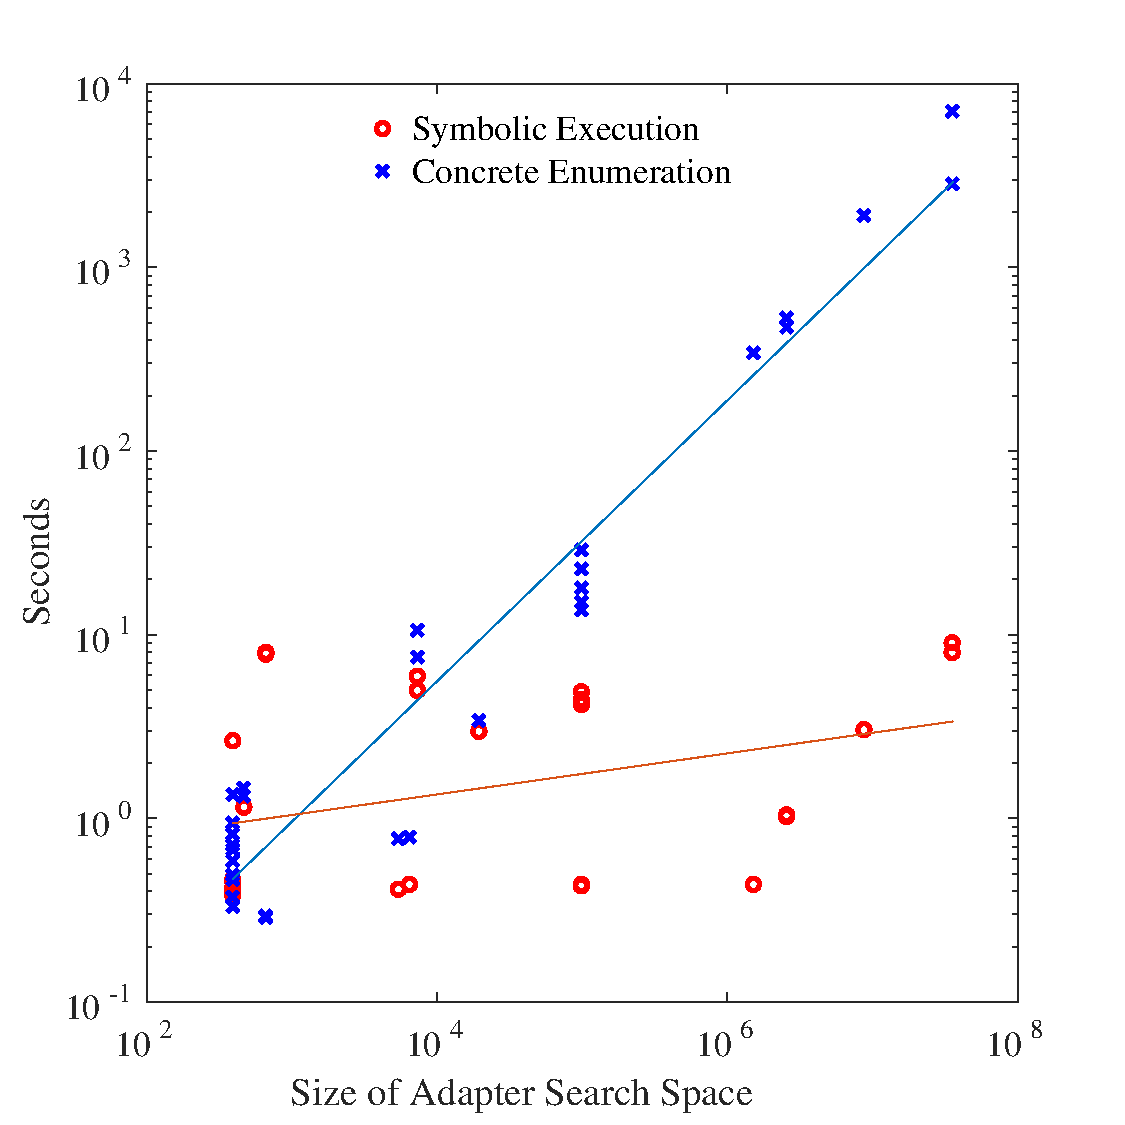
\includegraphics[width=\widthfactor\columnwidth]{chapters/adapter_synthesis/figures/conc_vs_se}
\end{figure}
%
For concrete enumeration-based adapter search, Figure~\ref{fig:conc_vs_se} shows the time required to find an adapter has a consistent exponential increase with an increase in the size of adapter search space.
%
But when using binary symbolic execution-based adapter search,
Figure~\ref{fig:conc_vs_se} shows a much slower increase in time
required to find the adapter.
%
This occurs because symbolic execution is less
affected by an increase in the size of the adapter search space
due to an increase in the number of arguments and the number of
possible constants in the adapter family.
%
\subsection{Large-Scale Reverse Engineering}
\label{subsec:eval_general}
In this section, we show how adapter synthesis can be used for reverse engineering.
Our goal is to understand the behavior of fragments of binary code by synthesizing adapters between those fragments and reference functions with known behavior.
We evaluate on binary code fragments taken from a ARM firmware image and reference functions
chosen from the source code of a popular media player.
\subsubsection{Code fragment selection}
Rockbox~\cite{rockbox} is a free replacement 3rd party firmware for digital music players.
%
We used a Rockbox image compiled for the iPod Nano (2g) device, based on the 32-bit ARM architecture, and disassembled it.
%
We dissected the firmware image into code fragments using the following rules:
%
(1) no code fragment could use memory, stack, floating-point, coprocessor, or supervisor call instructions,
%
(2) no code fragment could branch to an address outside itself,
%
(3) the first instruction of a code fragment could not be conditionally executed.

The first rule disallowed code fragments from having any inputs from/outputs to memory, thereby allowing us to use the 13 general purpose registers on ARM as inputs.
%
The second rule prevented a branch to an invalid address.
%
ARM instructions can be executed based on a condition code specified in the instruction. If the condition is not satisfied, the instruction is turned into a {\tt noop}.
%
The third rule disallowed the possibility of having code fragments that begin with a {\tt noop} instruction, or whose behavior depends on a condition.
%
The outputs of every code fragment were the last (up to) three registers written to by the code fragment.
%
This caused each code fragment to be used as the target code region up to three times, once for each output register.
%
This procedure gave us a total of 183,653 code regions, with 61,680 of them consisting of between 3 and 20 ARM instructions.

To evaluate which code fragments could be synthesized just with our
adapter family without a contribution from a reference function, we
checked
which of these 61,680 code fragments could be adaptably substituted by a reference function that simply returns one of its arguments.
%
Intuitively, any code fragment that can be adaptably substituted by an
uninteresting reference function must be uninteresting itself, and so
need not be considered further.
%
We found 46,831 of the 61,680 code fragments could not be adaptably
substituted by our simple reference function, and so we focused our
further evaluation on these 46,831 code fragments that were between 3
and 20 ARM instructions long and non-trivial.\\
%
\subsubsection{Reference functions}
Since our code fragments consisted of between 3 and 20 ARM instructions, we focused on using reference functions that can be expressed in a similar number of ARM instructions.
%
We used the source code of version 2.2.6 of the VLC media player~\cite{vlc} as the codebase for our reference functions.
%
We performed an automated search for functions that were up to 20 lines of source code.
%
This step gave us a total of 1647 functions.
%
Similar to the three rules for code fragment selection, we discarded functions that accessed memory, called other VLC-specific functions, or made system calls to find 24 reference functions.
%
Other than coming from a broadly similar problem domain (media
players), our selection of reference functions was independent of the
Rockbox codebase, so we would not expect that every reference function
would be found in Rockbox.

\subsubsection{Results}
We used the type conversion adapter family along with the return value
substitution family, disallowing return value substitution adapters
from setting the return value to be a type-converted argument of the
reference function (which would lead to uninteresting adapters).
%
We allowed the reference function arguments to be replaced by
unrestricted 32-bit constants, and we assumed each code segment takes
up to 13 arguments.
%
The size of this adapter search space can be calculated using the following formula:
\[8 \times \sum_{k=0}^{k=13} (2^{32})^{13-k} \times \comb{13}{k} \times \perm{13}{k} \times 8^k \]
%
The first multiplicative factor of 8 is due to the 8 possible return value substitution adapters.
%
The permutation and combination operators occur due to the choices of
arguments for the target code fragment and reference functions~(we
assumed both have 13 arguments since most general-purpose registers can
be used as input in an arbitrary code fragment).
%
The final $8^k$ represents the 8 possible type conversion operators that a type conversion adapter can apply.
%
The dominant factor for the size of the adapter search space comes from the size of the set of possible constants.
%
Our adapter family used unrestricted 32-bit constants, leading to a constants set of size $2^{32}$.

With this adapter family set up, we ran adapter synthesis trying to adaptably substitute each of the 46,831 code fragments by each reference function.
%
This gave us a total of 1,123,944~($46831 \times 24$) adapter synthesis tasks, with each adapter synthesis search space consisting of $1.353 \times 10^{127}$ adapters, too large for concrete enumeration.
%
%This calculation is using 10000 adapters concretely enumerated per second, which is a loose upper bound on what we observed when doing concrete adapter enumeration for popcnt.
%
We set a 5 minute hard time limit and a total memory limit of 2 GB per adapter synthesis task.
%
We split the adapter synthesis tasks for each reference function into 32 parallel jobs, creating a total of 768~($32 \times 24$) parallel jobs.
%
We ran our jobs on a machine cluster running CentOS 6.8 with 64-bit Linux kernel version 2.6.32 and Intel Xeon E5-2680v3 processors.
%
We present our results in Table~\ref{table:general}.
%
%The full set of results is presented in Section~\ref{sec:all_tables}.
%
%\input{chapters/adapter_synthesis/revengg_all_tables}
%
\input{chapters/adapter_synthesis/tables/revengg_general_compact}
The first column shows the reference functions chosen from the VLC media player source code.
%
The \textit{\#(full)} column reports how many code fragments were found to be adaptably substitutable~(represented by the value for \textit{\#}), and how many of those exploited the full generality of the reference function~(represented by the value of \textit{full}).
%
We report average number of steps and average total running time in the \textit{steps} and \textit{total time} columns respectively.
%
\subsubsection{Clustering using random tests} For every target code fragment and reference function pair, we can either find an adapter, find the fragment to not be adaptably substitutable, or run out of time.
%
Our adapter synthesis tool found adaptable substitution using 18 out of the 24 reference functions.
%
For every reference function, we clustered its adapted versions using 100,000 random tests. All adapted versions of a reference function that report the same output for all inputs were placed in the same cluster.
%
The number of clusters is reported in the \textit{\#clusters} column.
%
For each reference function, we then manually examined these clusters to judge which adapted versions used the complete functionality of that reference function; these are the cases where describing the functionality of the target fragment in terms of the reference function is mostly likely to be concise and helpful.
%
This took us less than a minute of manual effort for each reference function because we understood the intended semantic functionality of every reference function~(we had its source code).
%
We found instances of adapters using the full generality of the reference function for 11 reference functions.
%
Reference functions for which we found no use of full generality are omitted in Table~\ref{table:general}.
%
\begin{figure}
	\centering
	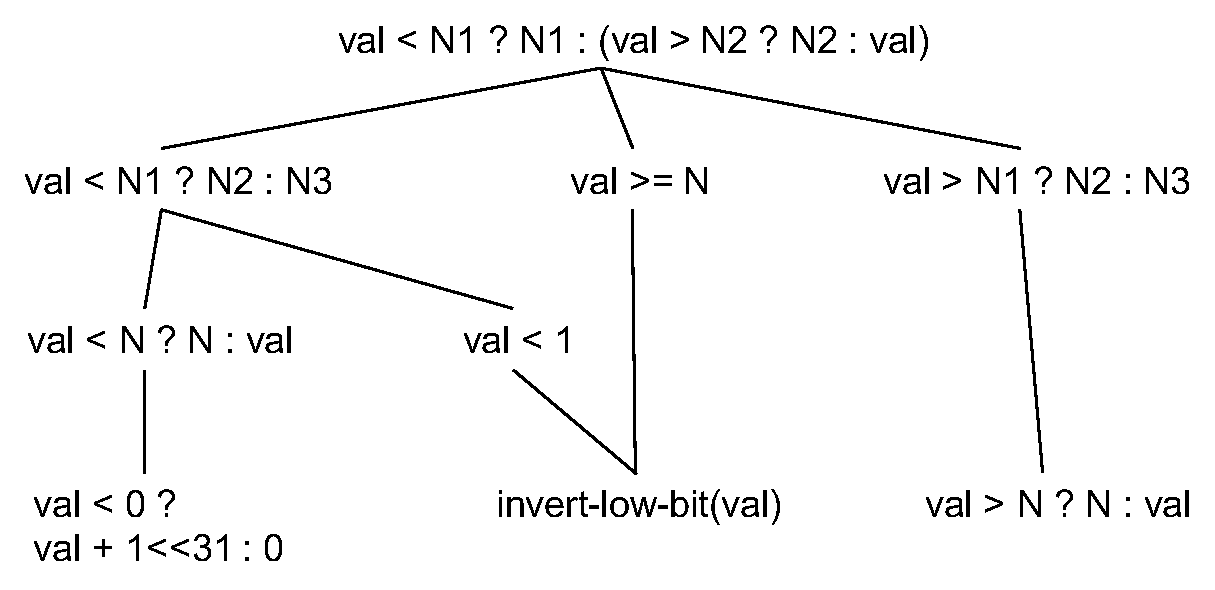
\includegraphics[width=\widthfactor\columnwidth]{chapters/adapter_synthesis/figures/clamp_partial_order}
	\caption{Subset of partial order relationship among adapted clamp instances}
	\label{fig:clamp_partial_order}
\end{figure}
We found that a majority of our generated adapters exploit specific functionality of the reference functions.
%
We explored this observation further by manually summarizing the semantics of the 683 adapters reported for {\tt clamp}.
%
We found that these 683 adapters have a partial order between them created by our adapter families of type conversion and return value substitution.
%
We present a subset of this partial order as a Hasse diagram in
Figure~\ref{fig:clamp_partial_order} with the most general
implementation of {\tt clamp} as the topmost node and functions that use
the most
specific instances of {\tt clamp} at the bottom.
%
To explain one unintuitive example, the {\tt invert-low-bit} operation on a value {\tt v} can be implemented in terms of {\tt val < N} by setting {\tt val} to the low bit of {\tt v} zero-extended to 32 bits and {\tt N} to 1, and zero-extending the low 1 bit of the return value of {\tt val < N} to 32 bits.
%
Some such functionalities owe more to the flexibility of the adapter
family than they do to the reference function.
%
These results suggest it would be worthwhile in the future to prune
them earlier by searching for instances of the simplest reference
functions first, and then excluding these from future searches.

Timeouts were the third possible conclusion of each adapter synthesis task.
The number of timeouts is reported in Table~\ref{table:general}.
%
We show a histogram of the total running time used to find adapters in Figure~\ref{fig:clamp_hist} for the {\tt clamp} reference function.
%
Similar histograms for {\tt tile\_pos} and {\tt median} reference
functions can be found in Section~\ref{sec:histograms}.
%
\input{chapters/adapter_synthesis/revengg_histograms}
%
\subsection{Comparing adapter families}
\label{sec:eval_compare}
%
We also explored the tradeoff between adapter search space size and effectiveness of the adapter family.
%
We ran all 46,831 target code fragments with {\tt clamp} as the reference function using two additional adapter families beyond the combination of type conversion family with return value substitution described above.
%
The first adapter family allowed only argument permutation and the second allowed argument permututation along with substitution with unrestricted 32-bit constants.
%
We ran the first adapter family setup (argument permutation + return value substitution) with a 2.5 minute hard time limit, the second adapter family setup (argument substitution + return value substitution) with a 5 minute hard time limit, and the third adapter family setup (argument substitution + return value substitution) was the same as the previous subsection with also a 5 minute hard time limit.
%
We present our results in Table \ref{table:compare}.
%
\begin{table}
\centering
\caption{Comparing adapter families with 46,831 target code fragments and {\tt clamp} reference function}
\label{table:compare}
\begin{tabular}{|l|l|l|l|l|}
\hline
																 & size           & \#-ad & \#-inequiv & \#-timeout \\ \hline
\begin{tabular}[c]{@{}l@{}}arg\_perm+\\ ret\_sub-2.5m\end{tabular} & 4.98E+10       & 9     & 46803      & 19         \\ \hline
\begin{tabular}[c]{@{}l@{}}arg\_sub+\\ ret\_sub-2.5m\end{tabular}  & 1.3538427E+126 & 705   & 45782      & 344        \\ \hline
\begin{tabular}[c]{@{}l@{}}type\_conv+\\ ret\_sub-5m\end{tabular}  & 1.3538430E+126 & 683   & 40553      & 5595       \\ \hline
\end{tabular}
\end{table}
%
As expected, the number of timeouts increases with an increase in the size of adapter search space.
%
Table \ref{table:compare} also shows that, for {\tt clamp}, a simpler adapter family is better at finding adapters than a more expressive family, because more searches can complete within the timeout.
%
But, this may not be true for all reference functions.
%
Table~\ref{table:compare} suggests that, when computationally feasible, adapter families should be tried in increasing order of expressiveness to have the fewest timeouts overall.
%
We plan to explore this tradeoff between expressiveness and effectiveness of adapter families in the future.



\section{Limitations and Future Work}\label{sec:discussion}
\label{sec:future_work}
%
%\todo{talk about inductive model checking}
%
%    To check equivalence of side-effects of the pair of functions on the operating system, our adapter synthesis tool checked for equality of a sequence of system call numbers.
%    %
%    Our equivalence checking can be extended to look for semantic, instead of exact, equivalence of system calls.
%    %But, again, comparing system call arguments for equivalence is not always as simple as checking for exact equality.
%    %For example, different invocations of the system call \textit{open} may be considered equivalent if they open the same file, even if the name of that file opened was read from a different address in memory.
%    %
%    In some cases, different system calls may be equivalent with certain parameters. 
%    %
%    For example, the \textit{creat} system call is equivalent to the \textit{open} system call with its second argument set to \textit{O\_CREAT|O\_WRONLY|O\_TRUNC}. 
%    %
%    Allowing for more relaxed notions of equivalence between system calls is non-trivial because of the many diverse side-effects that system calls can have on the filesystem and operating environment.
%    %
%    We can implement such side-effect equivalence checking by adding more thorough emulation of system call execution to FuzzBALL.
%    
%    Functions which use the same system calls can impose different preconditions on the system call arguments. 
%    %
%    e.g. we found that while the \textit{killpg} C library function internally calls the \textit{kill} function, it does this only if its first process group argument is greater than or equal to 0.
%    %
%    Adding knowledge of such preconditions to our adapter search can make our adapter synthesis implementation more robust but lies outside the scope of adapter synthesis.
%    %
%    While the presence of imposed pre-conditions can be detected from the implementation of a function, this problem becomes more difficult when functions use different values to represent the same semantic notion.
%    %
%    e.g. While \textit{isalpha} and \textit{isalnum} will return a non-zero value for an alphabetic character passed as an argument, they return different non-zero values to represent a boolean value \textit{true}. 
%    %
%    More expressive adapter grammars are required to be applied on the return value to allow synthesis of such post-conditions.


We currently represent our synthesized adapters by an assignment of concrete values to symbolic variables and manually check them for correctness. 
%
Adapters could instead be automatically incorporated into binary code to replace the original function with the adapted function.
%
This would make the adapters more convenient to use and easier to test automatically.
We plan to automate generation of such adapter code in the future.

During every adapter search step, symbolic execution explores all feasible paths, including paths terminated on a previous adapter search step because they did not lead to a correct adapter.
%
Once a candidate adapter is found, the next iteration of adapter search can be accelerated by using information saved from the previous iteration.
For example, adapter search can pick up symbolic execution from the last path in the previous iteration that led to a correct adapter.
%
A similar optimization can be utilized for concrete enumeration-based adapter
search that uses the same random order of adapters during an adapter
synthesis run. 
%
Concrete enumeration-based adapter search can be further accelerated by
searching for adapters in parallel since checking one adapter is
independent of checking other adapters.

%While we tested our adapter synthesis tool using the type conversion and argument substitution adapter grammars on a large number of function pairs, similar tests can be done for the arithmetic, argument substitution with string length, character set translation adapter grammars.
%
%
%
%Another interesting set of tests is to synthesize adapters between semantically equivalent functions in libraries that provide similar functionality.
%
%E.g. musl and glibc, the GNU C library, implement the standard library functionality.
%
%Synthesizing adapters between similar libraries can allow developers or users to swap one library with another.
%Preventing our memory-based equivalence checking from disqualifying adapters that find functional equivalence between functions that cleanup their writes to non-local memory would allow us to avoid false negatives during adapter search.
%We can also extend our adapter synthesis towards allowing certain parts of data structures present as part of the system state to be specified as symbolic which would allow exploration of more execution paths through the target and reference functions.
%
%e.g. using \textit{fputc} as the reference function with the lock variable within the file stream object set as symbolic would allow exploration of execution paths which depend on the lock already being acquired on the file. 
%
% Though our supported adapters are already useful, there are several directions in which we plan to extend them.
% %
% A simple extension is to allow floating-point values to be used with our type-conversion and arithmetic adapters.
% %
% A broader extension is to allow the user to specify operations allowed in adapters and to automatically translate the user\rq s specification into symbolic formulas. 
% %
% However, this can lead to the user specifying adapter search spaces that are too large.
% %
% Therefore, we would need to balance flexibility of user-guided adapter specifications with providing helpful guidance to the user on keeping the adapter search space within practical limits.
%
%For example, the C library function \textit{ether\_ntoa} can be replaced by an adapter which allocates a static buffer and passes it as the second argument to \textit{ether\_ntoa\_r}.
%
%We can also easily extend our adapter grammar to allow operations on floating point values. 
%adapter grammars which accommodate greater number of changes in function interfaces can also be developed and tested against functions in the C library.
%
%This would allow us to synthesize adapters between functions that implement mathematical formulas and between function pairs such as \textit{frexpf} and \textit{frexp}. 
%
%Adding type conversion operations to floating point adapter grammars would allow us to find argument substition adapters between function pairs such as \textit{frexpf} and \textit{frexp}.

Our tool currently assumes that all behaviors of the target function must be matched, modulo failures such as null dereferences.
%
Using a tool like Daikon~\cite{ernst2007daikon} to infer the preconditions of a function from its uses could help our tool find adapters that are only correct for correct uses of functions.
%
This would allow us to find equivalence between functions like {\em isupper} and {\em islower}, which expect certain types of input.

Adapter synthesis requires us to find if {\em there exists} an adapter such that {\em for all} inputs to the target function, the output of the target function and the output of the adapted reference function are equal. 
%
Thus the synthesis problem can be posed as a single query whose variables have this pattern of quantification (whereas CEGIS uses only quantifier-free queries).
%
We plan to explore using solvers such as Yices~\cite{yices} for this $\exists\forall$ fragment of first-order bitvector logic.

Symbolic execution can only check equivalence over inputs of bounded
size, though improvements such as path
merging~\cite{KuznetsovKBC2012,AvgerinosRCB2014} can improve scaling.
%
Our approach could also integrate with any other equivalence checking
approach that produces counterexamples, including ones that
synthesize inductive invariants to cover unbounded
inputs~\cite{SrivastavaG2009}, though we are not aware of any
existing binary-level implementations that would be suitable.


\section{Related Work}\label{sec:related-work}
\subsection{Detecting Equivalent Code}
%
The majority of previous work in this area has focused on detecting \emph{syntactically} equivalent code, or `clones,' which are, for instance, the result of copy-and-paste \cite{Kamiya:2002:CMT:636188.636191,Li:2004:CTF:1251254.1251274,Jiang:2007:DSA:1248820.1248843}. 
%
%Applications of detecting functionally equivalent code (aside from our motivating application of multivariant execution) include functionality-based refactoring, semantic-aware code search, and checking `yesterday's code against today's.'  
%
Jiang et al.~\cite{Jiang:2009:AMF:1572272.1572283} propose an algorithm for automatically detecting functionally equivalent code fragments using random testing and allow for limited types of adapter functions over code inputs --- specifically permutations and combinations of multiple inputs into a single struct. 
%Similar to our work, both \cite{Jiang:2009:AMF:1572272.1572283} and \cite{Ramos:2011:PLE:2032305.2032360} define functional equivalence based on input and output behavior. 
%The key difference between our approach and \cite{Jiang:2009:AMF:1572272.1572283} is that we rely on symbolic execution as opposed to random testing, and that we allow for more interesting adapter functions over code inputs. 
Ramos et al.~\cite{Ramos:2011:PLE:2032305.2032360} present a tool that checks for equivalence between arbitrary C functions using symbolic execution.
%
While our definition of functional equivalence is similar to that used by Jiang et al. and Ramos et al., our adapter families capture a larger set of allowed transformations during adapter synthesis than both. 

%Detecting pieces of equivalent code is useful for many applications including refactoring, code understanding, optimization, and plagiarism detection. 
%
Amidon et al.~\cite{program_fracture} describe a technique for fracturing a program into pieces which can be replaced by more optimized code from multiple applications.
%
They mention the need for automatic generation of adapters which enable replacement of pieces of code which are not immediately compatible.
%
While Amidon et al. describe a parameter reordering adapter, they do not mention how automation of synthesis of such adapters can be achieved.
%
David et al.~\cite{statistical_similarity} decompose binary code into smaller pieces, find semantic similarity between pieces, and use statistical reasoning to compose similarity between procedures.
%
Since this approach relies on pieces of binary code, they cannot examine binary code pieces that make function calls and check for semantic similarity across wrappers around function calls.
%
Goffi et al.~\cite{goffi} synthesize a sequence of functions that are equivalent to another function w.r.t a set of execution scenarios. 
%
Their implementation is similar to our concrete enumeration-based adapter search which produces equivalence w.r.t. a set of tests.
%
In the hardware domain, adapter synthesis has been applied to low-level combinatorial circuits by Gasc\'{o}n et al~\cite{gascon}.
%
They apply equivalence checking to functional descriptions of a low-level combinatorial circuit and reference implementations while synthesizing a correct mapping of the input and output signals and setting of control signals. 
%
They convert this mapping problem into a exists/forall problem which is solved using the Yices SMT solver~\cite{yices}. 
%
More recently, Katz et al.~\cite{katz2018rnn} have applied machine learning to the problem
of decompilation of binary code. 
%
Their technique predicts decompiled source code, given a fragment of
binary code.
%
A primary difference between adapter synthesis and the technique
presented by Katz et al. is that, if substitutability is found by
adapter synthesis, the match will be exact, whereas the Katz et al\rq s
technique finds an approximate match which may not be usable for
applications such as library replacement.
%
% Their permutation of input signals and output signals are similar to our argument substitution and return value adapters.
%
%However, their technique depends on the user specifying input and control signals for reference implementations whereas our technique does not depend on any such prior classification. 
%
%\subsection{Variant Generation}
%
%Another similar approach to developing variants relies on compiler-based randomization~\cite{Larsen:2014:SAS:2650286.2650803}. 
%
%It can be convenient to modify a compiler to support randomization because compilers already have support for many of the analyses required for randomization and are set up to target many different architectures. 
%
%However, compiler-based variant generation requires that the source code of the program to be randomized is available and that it is possible to customize the compiler. 
%
%Because we check for functional equivalence at the binary level, our approach does not require source code and is compatible with proprietary compilers. 
%
%Compiler-based approaches to diversity are also limited in the types of diversity they can introduce. 
%
\subsection{Component Retrieval}
%
Component retrieval is a technique~\cite{rittri},~\cite{runciman1989},~\cite{runciman1991} that provides a
search operator for finding a function, whose polymorphic type is known to the programmer, within a library of software components. 
%
The search results contain components whose types are similar but more general (or more specialized). 
%
Adapter synthesis shares the same intuition in that, it adapts the more
general implementation of a functionlity to the more specific one.
%
Type-based hot swapping~\cite{duggan} and signature
matching~\cite{zaremski} are related areas of research that rely on adapter-like operations such as currying or uncurrying functions, reordering tuples, and type conversion.
%
Reordering, insertion, deletion, and type conversion are only some of the many operations supported by our adapters. 
%
These techniques can only be applied at the source level, whereas our adapter synthesis technique can be applied at source and binary levels
%  
%  
%  
%  The earliest related work on type-based component retrieval was by Rittri~\cite{rittri}.
%  %
%  Given a query type A, Rittri presents a technique for searching through a library and finding all identifiers whose type is isomorphic to A.
%  This is done by modeling the problem as a Cartesian Closed Category (CCC) that has the product, exponentiation, and terminal objects defined and using products in normal forms as bags (multisets) which can then be compared for equality.
%  %
%  This paper actually mentions the need to have the search system provide a conversion function to convert the library value into the type of the user's query. 
%  %
%  This paper mentions work done by Runciman et al.~\cite{runciman1989} which allows the search system to include a search result where the library function has an extra argument which corresponds to a value that is constant in the user's application. 
%  %
%  These rules come together to form our argument substitution adapter family.
%  %
%  In an extended 1991 paper, Runciman et al.~\cite{runciman1991} present a technique for finding a function, whose polymorphic type is known to the programmer, within a library of software components. 
%  %
%  The technique was evaluated at the source level. 
%  %
%  The presented search operator allows a programmer to explore a library for near-misses, and presents the programmer with a list of search results. 
%  %
%  The search results contains components whose types are similar but more general (or more specialized). 
%  %
%  As mentioned by Runciman et al., their technique finds the curried form of a function that is more general, and is complementary to an approach that allows re-ordering, insertion, and deletion. 
%  %
%  However, re-ordering, insertion, and deletion are only some of the operations performed by our adapters. 
%  %
%  adapter synthesis is also related to type-based hot swapping of running modules in long-lived applications. 
%  %
%  Duggan~\cite{duggan} presents a technique for swapping modules while they are running where the swap must be type-based.%
%  This technique verifies the type-based swap to be correct on the basis of the version adapters provided by the user. 
%  %
%  The version adapters that this technique uses are exactly the same as our type conversion adapters. 
%  %
%  However, this technique depends on the version adapters being supplied for performing the type-based swap whereas our technique searches for the correct adapter. 
%  %
%  Signature matching is another problem which bears resemblance to adapter synthesis.
%  %
%  Zaremski et al.~\cite{zaremski} present a technique for finding functions or components in a library that match the user's query type. 
%  %
%  While an exact match of a search function type is useful, the technique can find more interesting search results by allowing for partial matches with relaxations such as generalized match, specialized match, and relaxations that allow transformations such as currying or uncurrying functions, reordering tuples. 
%  %
%  The reordering relaxation is similar to our argument substitution adapter family. 
%  %
%  Both of our techniques have similar applications, they lead to better program understanding, function reuse. 
%  %
%  However, our technique performs equivalence checking of the target and adapted reference functions, whereas their technique only matches type information. 
%  %
%  They mention that their technique can be combined with a specification matcher to search for specification matching only between function pairs that were returned as valid search results by their tool. 
%  %
%  Also, our technique is implemented at the binary level, whereas their technique is more likely to be useful as-is at the source level.

\subsection{Component Adaptation}
Component adaptation is another related area of research, that given a
formal specification of a query component, searches a library of
components within a set of adaptation architecture theories.
%
This includes techniques for adapter specification~\cite{nimble}, for component adaptation using formal specifications of components~\cite{spartacus},~\cite{penix},~\cite{penix1995},~\cite{yellin},~\cite{bracciali}.
%
Component adaptation has also been performed at the Java bytecode
level~\cite{keller}, as well as at low-level C code~\cite{nita}.
%
Behavior sampling~\cite{podgurski} is a similar area of research for finding equivalence over a small set of input samples.
%
However, these techniques either relied on having a formal specification of the behavior of all components in the library to be searched, or provided techniques for translating a formally specified adapter~\cite{nimble}.

%  One of the early works on component adaptation was by Purtilo et al.~\cite{nimble}.
%  %
%  They presented a language called Nimble which can be used by programmers to specify an interface adaptation for reuse of a module. 
%  %
%  The module reuse can be done in the same language or across different languages using module interconnection languages. 
%  %
%  This paper mentions the possibility of using an adapter function which performs the interface adaptation. 
%  %
%  The interface map is specified by the programmer and the code for the adapter function is generated by Nimble. 
%  %
%  This paper also mentions that if the bijection from the actual parameters passed by the calling function to the formal parameters taken by the reused function is order-preserving, such that the ith actual argument maps onto the ith formal argument, then the mapping is an isomorphism, and the parameter lists are syntactically equivalent. 
%  %
%  This is the definition used by the identity adapter which is the default adapter we start searching with.
%  %
%  The most significant difference between our work and Nimble is that Nimble requires the programmer to specify the adapter where we search for the adapter in an automated manner. 
%  %
%  If Nimble generated binary-level adapters, the adapters that our search tool finds could be encoded in the Nimble language and translated into binary code.
%  
%  A similar method of component adaptation was described by Morel et al.~\cite{spartacus}.
%  %
%  Given a formal specification of a component to be searched for and a library of components, SPARTACAS can automatically find an adaptation that reuses components in the library to implement the query component. 
%  %
%  SPARTACAS implements the adapter search using the sequential, alternative, and parallel adaptation architecture theories as described by Penix et al~\cite{penix}. 
%  %
%  Our adapter search technique can be extended further by implementing these adaptation architecture theories. 
%  %
%  For example, the sequential adaptation architecture can be used by passing the return value of one reference function as an argument to a second reference function.
%  %
%  The work done by Penix et al.~\cite{penix} is similar to adapter synthesis.
%  %
%  Penix et al. present a technique for automatic component adaptation using specification matching. 
%  %
%  The adaptation phase makes use of the results of a retrieval mechanism~\cite{penix1995} that classifies software components using semantic features derived from their formal specifications. 
%  %
%  The adaptation phase then searches for a way to adapt or combine components returned by the retrieval mechanism to solve the formal specification of a problem.
%  %
%  %
%  Formal approaches to component adaptation have also been proposed as presented by Yellin et al.~\cite{yellin} and extended by Bracciali et al.~\cite{bracciali}
%  %
%  These approaches adapt mismatched behavior between two components. 
%  %
%  Bracciali et al. provide a high-level notation for expressing adapter specifications, and an automated procedure for converting the adapter specifications to concrete adapters. 
%  %
%  Their work bears similarity to ours because they also express the adapter as a component-in-the-middle, similar to our intuition of the adapter being a wrapper around the reference function. 
%  %
%  Their one-to-one, many-to-one correspondence and use of the keyword none to indicate asymmetry between components when adapting components, were similar to the operations performed by our argument substitution adapter, when adapting functions. 
%  %
%  Finally, both our technique and theirs perform adaptation at the interface level.
%  %
%  However, our technique adapts the reference function to the target function, whereas their technique adapted mismatched behavior between both components simultaneously. 
%  %
%  Our technique treats the binary-level implementation of the target and reference functions as their own behavior specification whereas their technique requires the behavior of both components to be formally specified. 
%  %
%  Our adaptation technique does not depend on the availability of formal specifications of functions and, therefore, is an improvement over the work presented in these component adaptation techniques.
%  
%  Component adaptation has also been done at the Java bytecode level~\cite{keller}.
%  %
%  In this work, the programmer writes a delta (adapter) specification, which is translated into a modified class bytecode form by a Delta compiler. 
%  %
%  The allowed operations are renaming of class, methods, fields, changing the super class, add interface to implements clause, add method, add field to the class, and finally, rename a symbolic reference to a field. 
%  %
%  Java byte code contains all references to classes, interfaces, and fields, type information of all methods, method names, to ensure safe execution of programs. 
%  %
%  The adaptation is done only if the previously-specified preconditions are met. 
%  %
%  Thus, adapter search is not automated, but manually defined in an earlier step (adapter specification).
%  %
%  Adaptation of data layout has also been done at the bit-level for C code by Nita et al~\cite{nita}.
%  %
%  However, this work also allows a programmer to specify multiple alternative data layouts in a declarative language, instead of automating this search.
%  
%  Behavior sampling~\cite{podgurski} also bears a similarity with adapter synthesis.
%  %
%  This technique includes our intuition that the order of parameters is not important as long as there is one-to-one correspondence between the parameters of the target interface and the formal parameters of the reference interface and the correspondence also respects types and modes.  
%  %
%  This technique finds behavioral equivalence over a small set of input samples and leaves it up to the user to determine exact equivalence by going through the search results. 
%  %
%  The user must also define expected outputs for each input in the sample set by computing the output values by hand or some other means. 
%  %
%  This is in contrast with our technique which finds exact equivalence over all inputs to the target function where the reference function is being adapted to become behaviorally equivalent to the target functions.
%  % 
\subsection{Program Synthesis}
%
Program synthesis is an active area of research that has many applications including generating optimal instruction sequences \cite{Massalin:1987:SLS:36206.36194,Joshi:2002:DGS:512529.512566}, automating repetitive programming, filling in low-level program details after programmer intent has been expressed \cite{Solar-LezamaTBSS2006}, and even binary diversification \cite{Jacob2008}. 
%
Programs can be synthesized from formal specifications \cite{Manna:1980:DAP:357084.357090}, simpler (likely less efficient) programs that have the desired behavior \cite{Massalin:1987:SLS:36206.36194,Solar-LezamaTBSS2006,Joshi:2002:DGS:512529.512566}, or input/output oracles \cite{Jha:2010:OCP:1806799.1806833}. 
%
We take the second approach to specification, treating existing functions as specifications when synthesizing adapter functions.
%
% We focus on a type of synthesis known as counterexample-guided inductive synthesis (CEGIS). 
% CEGIS is useful for our work because it is guaranteed to terminate when the space of possible programs is finite, and if it terminates by producing a program, then that program is guaranteed to be correct with respect to the specification. 
% Though the space of candidate programs may be very large, a CEGIS search tends to take relatively few iterations \cite{Solar-LezamaTBSS2006}.
% 
% 
% 
%    \subsection{$N$-version Systems}
%    %\subsection{$N$-version and $N$-variant Systems}
%    The earliest work related to creating function equivalence happened during the 1970s when fault-tolerant computing research began to gain momentum and the idea of n-version programming was proposed~\cite{chen1977},~\cite{chen1978}.
%    N-version programming is defined as the process of independently generating functionally equivalent programs from the same initial specification.
%    Since then, a variety of work has analyzed the assumption of the independence of errors among different versions \cite{Knight:1986:EEA:10677.10688}, the effectiveness of $N$-version programming in the presence of overlapping errors \cite{Eckhardt:1985:TBA:1314034.1314066}, and the practicality from a software engineering standpoint of developing multiple less-reliable versions versus a single highly-reliable version \cite{Hatton:1997:NDV:624622.625783}. 
%    %Generally, this work finds that running several program versions simultaneously and using a voting mechanism can produce a system that is more reliable than any of the versions individually, and that developing different versions of a program is a good way to achieve fault tolerance considering that it is difficult to develop one really good, bug-free version. 
%    %However, this work also suggests that it is difficult to make formal guarantees about the security that an $N$-version system provides.
%    
%    Recent approaches~\cite{Baudry:2015:MFS:2808687.2807593} to $N$-version programming have taken advantage of \emph{natural diversity} seen in related software programs. 
%    Natural diversity refers to diverse implementations of the same functionality that emerge naturally, typically due to economic competition. 
%    Natural diversity can be seen in the diverse implementations of, but similar functionalities provided by, Web browsers, operating systems, firewalls, database management systems, and so on. 
%    Studies have shown that the naturally-emerging diverse implementations of different commercial-off-the-shelf products are good candidates for $N$-version programming because they typically have independent bugs \cite{Gashi:1311908, Han:2009:ESD:1575533.1575544}. 
%    %We hope to take advantage of natural diversity within a codebase when looking for functionally equivalent functions.
%    
%    %Another recent take on the idea of executing multiple implementations of a program simultaneously for fault tolerance is called $N$-variant (or multivariant) execution \cite{Cox:2006:NSS:1267336.1267344,Salamat:5714703}. 
%    %The distinction between a `version' and a `variant' is that a version is manually developed while a variant is automatically generated. 
%    %Cox et al.~\cite{Cox:2006:NSS:1267336.1267344} show how to construct variants, so that they have disjoint vulnerabilities with respect to certain classes of attacks, using two randomization techniques: memory address partitioning, which provides protection against attacks involving absolute memory addresses, and instruction tagging, which detects attempts to execute injected code. 
%    %Salamat et al.~\cite{Salamat:5714703} introduce a user-space multivariant execution environment (MVEE) that monitors multiple variants of a program running in parallel and show that this technique is effective in detecting and preventing code injection attacks. 
%    %MVEE variants are generated using different stack growths and system call number randomization. One restriction to the MVEE is that it requires all variants to make the same system calls, in the same order, with the same arguments.
%    %
%    %Automated variant construction avoids the overhead of manual development of multiple program versions and enables more formal arguments about a system's security, but existing variant construction techniques are limited in the types of diversity that they can introduce. 
%    %Techniques like memory address partitioning, instruction tagging, memory rearrangement, and system call randomization do not introduce diversity at the design level, i.e. at the level of data structures and algorithms. 
%    %We believe that design-level diversity is also an important source of protection against attacks and we hope to discover design-level diversity through our search for equivalent functions. 
%    %However, to avoid the cost of manually developing different program implementations, we want to use the diverse equivalent functions we find in an automated way. 
%    
%    %A discussion of how to automate construction of program variants using equivalent function implementations is beyond the scope of this paper, but we mention briefly that there are many possible approaches. 
%    %For example, we could take a static rewriting approach and randomly replace function calls at the source code or binary level by other equivalent function calls with appropriately modified arguments. 
%    %Or we could take a dynamic approach and replace function calls during run time.
%    


\section{Conclusion}\label{sec:conclusion}
%
We presented a new technique to search for semantically-equivalent pieces of code which can be substituted while adapting differences in their interfaces.
%
This approach is implemented at the binary level, thereby enabling wider applications and consideration of exact run-time behavior.
%
We implemented adapter synthesis for x86-64 and ARM binary code.
%
We presented examples demonstrating applications towards adaptation modulo a bug, library replacement, and reverse engineering. 
%
We present an evaluation to find substitutable code within a library using the C library.
%
Our adapter families can be combined to find sophisticated adapters as shown by adaptation of RC4 implementations.
%
While finding thousands of functions to not be equivalent, our tool reported many instances of semantic equivalence, including C library functions such as \textit{ffs} and \textit{ffsl}, which have assembly language implementations.
%
Our comparison of concrete enumeration-based adapter search with binary
symbolic execution-based adapter search allows users of adapter
synthesis to choose between the two approaches based on the size of the adapter search space.
%
Our case studies show that adapter synthesis can be applied at scale to reverse engineer binary code using independently-developed codebases, even in the presence of very large adapter search spaces. 
%
Our implementation constitutes a novel use of  binary symbolic execution for synthesis.
%
Our results show that the CEGIS approach for adapter synthesis of binary code is feasible and sheds new light on potential applications such as searching for efficient clones, deobfuscation, program understanding, and security through diversity.
%

%    We have presented a new approach for finding code segments which are
%    semantically substitutable despite having different interfaces.
%    %
%    The approach works by automatically finding the wrapper code (adapter)
%    that would allow one code segment to replace another, or proving that
%    no such adapter exists from a given grammar.
%    %
%    The technique is implemented using symbolic execution, so it considers
%    precise code behavior without needing to execute every concrete
%    function input separately, and it can search over binaries without
%    requiring source code.
%    %
%    We implement the technique for x86-64 machine code, and apply it to
%    over 13,000 function pairs within the C library on a Linux system,
%    where it finds dozens of semantically-equivalent functions while
%    proving that thousands of others are not equivalent.
%    %
%    Though this case study only illustrates one possible application of
%    the technique, it already shows that it scales to run automatically
%    over a large and diverse code base and finds adapters which we confirm
%    to be correct.
%    %
%    This suggests that adapter synthesis is a promising approach for
%    semantic clone search that accounts for the interface diversity of
%    real software.


%\newpage
%    \section{Acknowledgements}\label{sec:acknowledgements}
%    We would like to acknowledge DARPA and NSF for funding this research. 
%    %
%    We would like to thank Stephen McCamant for his many helpful discussions and feedback during the course of this research.
%    %
%    We wish to thank Kesha Hietala for her helpful suggestions during experimental setup and design of adapter grammars.
%    %
%    We also wish to acknowledge the computing infrastructure made available to us by the Minnesota Supercomputing Institute.

%\input{chapters/adapter_synthesis/new_appendix}


%%%%%%%%%%%%%%%%%%%%%%%%%%%%%%%%%%%%%%%%%%%%%%%%%%%%%%%%%%%%%%%%%%%%%%%%%%%%%%%%

%%%%%%%%%%%%%%%%%%%%%%%%%%%%%%%%%%%%%%%%%%%%%%%%%%%%%%%%%%%%%%%%%%%%%%%%%%%%%%%%
% path_merging_connection.tex: Chapter describing the experiment
%%%%%%%%%%%%%%%%%%%%%%%%%%%%%%%%%%%%%%%%%%%%%%%%%%%%%%%%%%%%%%%%%%%%%%%%%%%%%%%%
\chapter{Using Path-merging With Adapter Synthesis}
\label{path_merging_connection_chapter}
%%%%%%%%%%%%%%%%%%%%%%%%%%%%%%%%%%%%%%%%%%%%%%%%%%%%%%%%%%%%%%%%%%%%%%%%%%%%%%%%


%Software Chapters
%%%%%%%%%%%%%%%%%%%%%%%%%%%%%%%%%%%%%%%%%%%%%%%%%%%%%%%%%%%%%%%%%%%%%%%%%%%%%%%%
%adapter_synthesis.tex: Chapter on adapter synthesis
%%%%%%%%%%%%%%%%%%%%%%%%%%%%%%%%%%%%%%%%%%%%%%%%%%%%%%%%%%%%%%%%%%%%%%%%%%%%%%%%
\chapter{Java Ranger: Static Regions For Efficient Symbolic Execution Of Java}
\label{java_ranger_chapter}
%%%%%%%%%%%%%%%%%%%%%%%%%%%%%%%%%%%%%%%%%%%%%%%%%%%%%%%%%%%%%%%%%%%%%%%%%%%%%%%%



%Path explosion problem is still the main obsticale against scaling up symbolic execution to industrial sized projects.
%%
%One interesting resolution to the problem is \emph{Veritesting}, which represents regions of code as disjunctive formals over paths.
%%
%Unlike the C compiler that inlines functions in programs, Integrating veritesting with Java bytecode presents unique challenges: notably, incorporating non-local control jumps caused by runtime polymorphism, exceptions, native calls, and dynamic 3 class loading.
%%
%In this paper we present our robust implementation of Java based veritesting tool that supports dynamic dispatch and
\section{Introduction}
%
Symbolic execution is a popular analysis technique that performs non-standard execution of a program: operations
in the program generate formulas over inputs along every feasible execution through branches in the program, and
branch constraints along an execution path are combined into a predicate.
%
Originally developed in the 1970s~\cite{King1976,Clarke1976}, symbolic execution is a convenient building block for
program analysis, since arbitrary behavior in the program can be discovered by adding query predicates for it to
the symbolic program representation, and solutions to these constraints are inputs that provide the queried behavior in the program.
%
Some of the applications of symbolic execution include
test generation~\cite{dart,cute}, equivalence checking~\cite{ramos,adaptorsynth}, vulnerability finding~\cite{driller,angr}, and protocol correctness checking~\cite{transport}.
%
Symbolic execution tools are available for many languages, including
CREST~\cite{BurnimS2008} for C source code, KLEE~\cite{CadarDE2008}
for C/C++ via LLVM, JDart~\cite{jdart2016} and Symbolic
PathFinder (SPF)~\cite{spf} for Java, and S2E~\cite{ChipounovKC2012},
FuzzBALL~\cite{BabicMMS2011}, and {\tt angr}~\cite{angr}, FuzzBALL~\cite{fuzzball} for binary code.
%
%Some of these tools, such as {\tt angr} and Mayhem~\cite{mayhem} that operate at the binary-level, are used for finding
%security bugs.
%
%Others, such as KLEE, are used for exploring system-level programs for software engineering purposes.

% \mike{More here...explain the `ecosystem' - tools for different languages: KLEE, FuzzBall, Java Symbolic Pathfinder, ...}

However, scalability remains a significant challenge for many applications of symbolic execution.
%
In particular symbolic execution can suffer from a {\em path explosion}: every symbolic branch that has two feasible sides
causes the number of execution paths that need to be explored to be multiplied by two.
%
Real-world software tends to have many branches, thereby creating exponentially many execution paths.
%
Symbolic execution techniques that explore one path at a time are unable to cover all paths within a reasonable time budget.
%
Dynamic state merging~\cite{HansenSS2009,kuznetsov} provides one way to
alleviate scalability challenges by merging dynamic
symbolic executors, effectively merging the paths they represent, when the benefit of introducing new symbolic state
heuristically outweighs its cost.
%
Veritesting~\cite{veritesting} is another path-merging technique that can dramatically improve the performance of
symbolic execution by effectively merging paths.
%
Rather than explicitly merging state representations, veritesting represents a local region of a program containing
branches as a disjunctive summary for symbolic analysis.
%
This often allows many paths to be collapsed into a single path involving the region.
%
In previous work~\cite{veritesting}, constructing such bounded static summaries was shown to allow symbolic execution to
find more bugs, and achieve more node and path coverage, when implemented at the X86 binary level for compiled C programs.
%
This motivates investigation using static regions for symbolic execution of Java software (at the Java bytecode level).

Java programmers who follow best software engineering practices attempt to write code in an object-oriented
form with common functionality implemented as a Java class and multiple not-too-large methods used to implement small
sub-units of functionality.
%
This causes Java programs to make several calls to methods, such as getters and setters, to re-use small common sub-units
of functionality.
%
Merging paths within regions in such Java programs using techniques described in current literature is limited by not having the ability
to inline method summaries.
%
This is not a major impediment for compiled C code, as the C compiler will usually automatically inline the code for short
methods such as \texttt{get}.
%
However, Java has an {\em open world} assumption, and most methods are {\em dynamically dispatched}, meaning that the code to be
run is not certain until a method is resolved at runtime; if inlining is performed at all, it is by the JRE, so it is not reflected in bytecode.

One feature commonly used by Java developers is the use of fields and arrays in Java code.
%
Summarizing non-static field accesses requires finding which object a field access belongs to, an operation which
cannot be computed exactly in a static analysis.
%
Instead of summarizing field accesses statically, our interpretation of path-merging for Java code regions computes
such a summary only when a summary is instantiated by the symbolic executor.
%
A further generalization of this problem arises with symbolic index-based accesses into array objects.
%
Our interpretation of path-merging supports symbolic indices, by including the possibility of any entry in the array
being accessed, in the region\rq s summary.
%
A couple of other improvements in our path-merging technique include include summaries of methods and supporting
exceptional behavior in regions.

Not being able to summarize such dynamically dispatch methods can lead to poor performance for
n\"aive implementations of bounded static regions.
%
Thus, to be successful, we must be able to inject the static regions associated with the calls into the dispatching
region.
%
We call such regions {\em higher order} as they require a region as an argument and can return a region that may need
to be further interpreted.
%
In our experiments, we demonstrate exponential speedups on benchmarks (in general, the more paths contained within a
program, the larger the speedup) over the unmodified Java SPF tool using this approach.

Another common feature of Java code that represents the boundary of path merging is \textit{exceptions}.
%
If an exception can potentially be raised in a region, the symbolic executor needs to explore that exceptional behavior.
%
But, it is possible for other unexceptional behavior to also exist in the same region.
%
For example, it can be in the form of a branch nested inside another branch that raises an exception on the other side.
%
Summarizing such unexceptional behavior while simultaneously guiding the symbolic executor towards potential exceptional
behavior reduces the branching factor of the region.
%
We propose a technique named \textit{Single-Path Cases} for splitting a region summary into its exceptional and
unexceptional parts.

While summarizing higher-order regions and finding single-path cases is useful to improve scalability,
representing such summaries in an intermediate representation~(IR) that uses static single-assignment~(SSA) form
provides a few key advantages.
%
(1) It allows region summaries to be constructed by using a sequence of transformations, with each transformation
extending to add support for new features such as heap accesses, higher-order regions, and single-path cases.
%
(2) It allows for simplifications such as constant propagation, copy propagation, constant folding to be performed on
region summaries.
%
(3) It makes the construction of region summaries more accessible to users of the symbolic execution tool, thereby making
path merging more useful to end-users.\\
%
In this chapter, we present Java Ranger, an extension of Symbolic PathFinder, that computes such region summaries over a representation we call
Ranger IR.
%
Ranger IR has support for inlining method summaries and for constructing SSA form for heap accesses.
%
It also proposes Single-Path Cases as an alternative to multiple transition points as
defined by Avgerinos et al.~\cite{veritesting}.


\subsection{Motivating Example}
\begin{figure}
    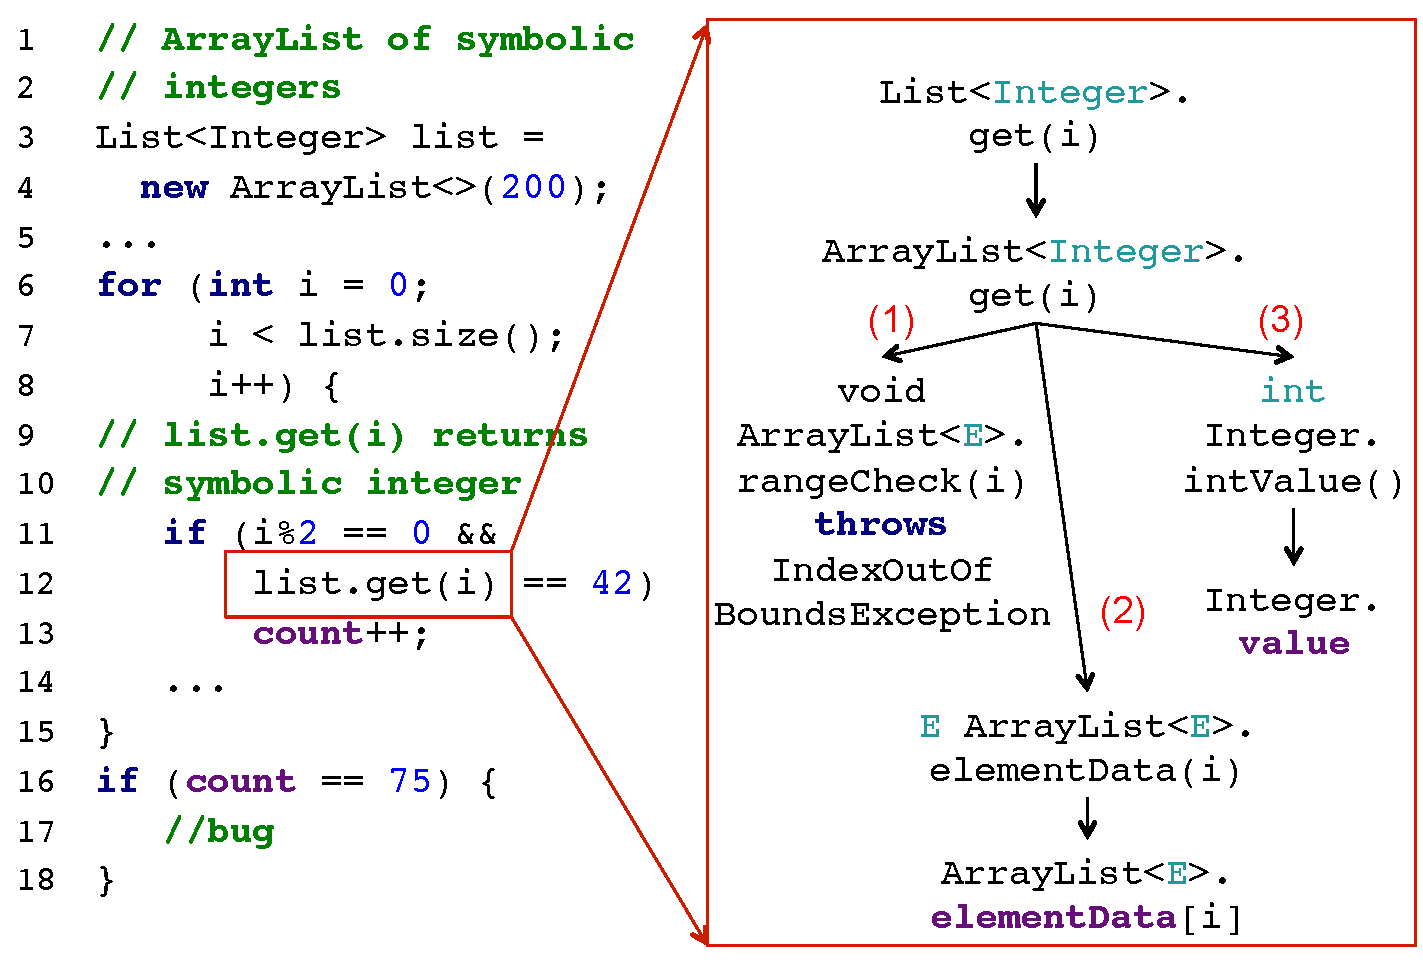
\includegraphics[width=\widthfactor\textwidth]{chapters/java_ranger/figures/example-combined.pdf}
    \caption{An example demonstrating the need for using a multi-path region summary}
    \label{fig:mot-example}
\end{figure}
Consider the example of Java code shown in Figure \ref{fig:mot-example}.
%
The {\tt list} object refers to an {\tt ArrayList} of 200 {\tt Integer} objects which have an unconstrained symbolic
integer as a field.
%
The checking of each even-indexed entry in {\tt list} introduces a branch, which has both sides feasible, and requires
symbolic execution to explore two execution paths instead of the one it was at.\\
%
Performing this check over the entire {\tt list} makes symbolic execution need $2^{100}$ execution paths to terminate
(assuming {\tt list} has 200 entries with every even-indexed entry pointing to a new unconstrained symbolic integer).
%
A simple way to avoid this path explosion is to merge the two paths arising out of the {\tt i\%2 == 0 \&\& list.get(i) == 42} branch.
%
Such path merging requires us to compute a summary of all behaviors arising on both sides of the branch from lines 11 to 13
until both sides of the branch merge at line 14.
%
If we can construct such a summary beforehand, our symbolic executor can instantiate the summary by reading in inputs to
the summary from the stack and/or the heap, and writing outputs of the summary to the stack and/or the heap.\\
%
Unfortunately, constructing such a summary for this simple region from lines 11--13 is not straightforward due to the
call to {\tt list.get(int)} which is actually a call to {\tt ArrayList<Integer>.get(int)} ({\tt java.util.List<E>.get(int)} is abstract and does not have an implementation).
%
{\tt ArrayList<Integer>.get(int)} internally does the following:
%
\begin{enumerate}
\item It checks if the index argument accesses a value within bounds of the {\tt ArrayList} by calling {\tt ArrayList<E>.rangeCheck(int)}. If this access is not within bounds, it throws an exception.
%
\item It calls {\tt ArrayList<E>.elementData(int)} to access an internal array named {\tt elementData} and get the entry at position {\tt i}. This call results in an object of class {\tt Integer} being returned.
%
\item It calls {\tt Integer.intValue()} on the object returned by the previous step. This call internally accesses the {\tt value} field of {\tt Integer} to return the integer value of this object.
%
\end{enumerate}

The static summary of {\tt ArrayList<Integer>.get(int)} needs to not only include summaries of all these three methods but
also include the possibility of an exception being raised by the included summary of {\tt ArrayList<E>.rangeCheck(i)}.
%
Our extension to path-merging includes using method summaries, either with a single return or no return, as part of region summaries that have method calls \footnote{We plan to support methods with multiple returns in the future.}.
%
The method whose summary is to be included depends on the dynamic type of the object reference on which the method is being invoked.
%
In our example, the dynamic type of {\tt list} is {\tt ArrayList}, whereas it is declared statically as having the type {\tt List}.
%
Therefore, the summary of {\tt list.get(i)} pulls in the method summaryof {\tt ArrayList<E>.get(i)}.\\
%
Our \textit{Single-Path Cases} extension to path-merging also allows the possibility of exceptional behavior being
included in the summary and explored separately from unexceptional behavior by performing exploration of exceptional
behavior in the region on its own execution path.
%

%\input{preliminaries}
%\input{challenges}
\section{Related Work}
\todo[inline]{Rewrite this section in your own words}
Path explosion is a major cause of scalability limitations for
symbolic execution, so an appealing direction for optimization is to
combine the representations of similar execution paths, which we refer
to generically as {\em path merging.}
%
If a symbolic execution tool already concurrently maintains objects
representing multiple execution states, a natural approach is to merge
these states, especially ones with the same control-flow location.
%
Hansen et al.~\cite{HansenSS2009} explored this technique but found
mixed results on its benefits.
%
Kuznetsov et al.~\cite{kuznetsov} developed new algorithms and
heuristics to control when to perform such state merging profitably.
%
A larger departure in the architecture of symbolic execution systems
is the MultiSE approach proposed by Sen et al.~\cite{multise}, which
represents values including the program counter with a two-level
guarded structure, in which the guard expressions are optimized with
BDDs.
%
The MultiSE approach achieves effects similar to state merging
automatically, and provides some architectural advantages such as in
representing values that are not supported by the SMT solver.

Another approach to achieve path merging is to statically summarize
regions that contain branching control flow.
%
This approach was proposed by Avgerinos et al.~\cite{veritesting} and
dubbed ``veritesting'' because it pushes symbolic execution further
along a continuum towards all-paths techniques used in verification.
%
A veritesting-style technique is a convenient way to add path merging
to a symbolic execution system that maintains only one execution
state, which is one reason we chose it when extending SPF.
%
Avgerinos et al. designed and implemented their veritesting system
MergePoint for the application of binary-level symbolic execution for
bug finding.
%
They found that veritesting provided a dramatic performance
improvement, allowing their system to find more bugs and have better
node and path coverage in a given exploration time.
%
The static regions used by MergePoint are intra-procedural, but they
can have any number of ``transition points'' at which control can be
returned to regular symbolic execution.
%
Avgerinos et al. do not provide details about how MergePoint
represents memory accesses or integrates them with veritesting, though
since MergePoint was built as an extension of the same authors' Mayhem
system, it may reuse techniques such as symbolic representation of
loads from bounded memory regions~\cite{mayhem}.

The veritesting approach has been integrated with another binary level
symbolic execution engine named {\tt angr}~\cite{angr}.
%
However angr's authors found that their veritesting implementation did
not provide an overall improvement over their dynamic symbolic
execution baseline: though veritesting allowed some new crashes to be
found, they observed that giving more complex symbolic expressions
slowed down the SMT solver enough that total performance was degraded.
%
We have also observed complex expressions to be a potential cost of
veritesting, but we believe that optimizations of the SMT solver
interface and potentially heuristics to choose when to use static
regions can allow them to be a net asset.

The way that \tool\ and similar tools statically convert code
regions into formulas is similar to techniques used in verification.
%
In the limit where all relevant code in a program can be
summarized, such as with WBS and TCAS-SR in Section~\ref{sec:results},
\tool\ performs similarly to a bounded symbolic model checker for
Java.
%
SPF and \tool\ build on Java Pathfinder (JPF)~\cite{jpf}, which is
widely used for explicit-state model checking of Java and provides
core infrastructure for instrumentation and state backtracking.
%
Another family of Java analysis tools that use formula translation
(also called verification condition generation) are
ESC/Java~\cite{FlanaganLLNSS2002}, ESC/Java2~\cite{CokK2004}, and
OpenJML~\cite{Cok2011}, though these tools target static error
checking and verification of annotated specifications.

Perhaps the most closely related Java model checking tool is
JBMC~\cite{CordeiroKKST2018}, which has recently been built sharing
infrastructure with the similar C tool CBMC.
%
JBMC performs symbolic bounded model checking of Java code,
transforming code and a supported subset of the standard library into
SMT or SAT formulas that represent all possible execution paths.
%
(The process by which JBMC transforms its internal code representation
into SMT formulas is sometimes described as (static) symbolic
execution, but it has more in common with how \tool\ constructs static
regions than with the symbolic execution that vanilla SPF performs.)
%
In cases that \tool\ can completely summarize, we would expect its
performance to be comparable to JBMC's; an experimental comparison is
future work.
%
But static region summaries are more important as an optimization to
speed up symbolic execution on software that is too large and/or
complex to be explored exhaustively.

A wide variety of other enhancements to symbolic execution have been
proposed to improve its performance, including caching and simplifying
constraints, summarizing repetitive behavior in loops, heuristic
guidance towards interesting code, pruning paths that are repetitive
or unproductive, and many domain-specific ideas.
%
A recent survey by Baldoni et. al.~\cite{SurveySymExec-CSUR18}
provides pointers into the large literature.
%
One approach that is most related to our higher-order static regions
is the function-level compositional approach called SMART proposed by
Godefroid~\cite{Godefroid2007}.
%
Like \tool's function summaries, SMART summarizes the behavior of a
function in isolation from its calling context so that the summary can
be reused at points where the function is used.
%
But SMART uses single-path symbolic execution to compute its
summaries, whereas \tool\ uses static analysis: this makes \tool's
summary more compact at the expense of requiring more reasoning by the
SMT solver.
%
Because SMART was implemented for C, it does not address dynamic
dispatch between multiple call targets.


% %Talk about other symbolic execution performance improvements.
% %mentioned in Christopher Kruegel's ISSTA keynote talk as Static Analysis support
% Other static analysis techniques also provide support for dynamic symbolic execution.
% %
% Loop-extended symbolic execution introduced partial loop summarization by having symbolic variables that represent the number of times each loop executes.
% %
% This technique allowed symbolic variables to incorporate loop dependent effects along with data dependencies from program inputs.
%
%Value Set Analysis~\cite{vsa} is another static analysis technique that can potentially benefit dynamic symbolic execution.
%%
%Value set analysis uses an abstract domain to find an over-approximated set of values that registers or abstract locations may have at program points.
%%
%Value set analysis can help dynamic symbolic execution resolve ranges without solving constraints.
%VSA can resolve ranges without solving constraints, thereby, finding applications in computing all possible write targets during a memory write operation.
%Code summarization (Dodo)
%  - automatically (and statically) summarize effect of loops / functions
%VSA - value set analysis
%  - resolve ranges (and conditionals) without solving constraints

%Talk about TamiFlex, and how using the same technique as TamiFlex is one way to solve veritesting challenges in Java bytecode.
%
%Other techniques for static analysis at the Java bytecode level can also benefit dynamic symbolic execution.
%
%Finding which reflective method call is being used, or handling dynamic class loading are known problems for static analysis tools.
%
%TamiFlex~\cite{tamiflex} provides an answer that is sound with respect to a set of previously seen program runs.
%
%Integrating veritesting runs into similar problems, and using techniques from TamiFlex would allow static predicate construction beyond exit points caused by reflection or dynamic class loading. 

\section{Technique}
%
To add path merging to SPF, we first pre-compute static summaries of arbitrary code regions with more than one execution
path and we also pre-compute method summaries.
%
To bound the set of code regions we analyze, we start by specifying a method $M$ in a configuration file.
%
Next, we construct a set containing only the class $C$ that contains $M$.
%
We then get another set of classes, $C'$,
such that every class in $C'$ has at least one method that was called by a method in a class in $C$.
%
This step which goes from $C$ to $C'$ discovers all the classes at a call depth of 1 from $C$.
%
We continue this method discovery process up to a call depth of 2.
%
While we can increase the call depth in our method discovery process, we found that summarizing
arbitrary code regions with more than 2 calls deep, did not lead to practically useful region summaries.
%
After obtaining a list of methods, we computed static summaries of regions in these methods and method summaries as
explained in Section \ref{sec:static-analysis}.
%
After computing static region and method summaries, we process them as a sequence of transformations described in the next section~\ref{sec:instantiationTransformations} and summarized
in Figure~\ref{fig:overview}.
%
\begin{figure}[]
    \caption{Overview of transformations on Ranger IR to create and instantiate multi-path region summaries with higher-order regions}
    \label{fig:overview}
    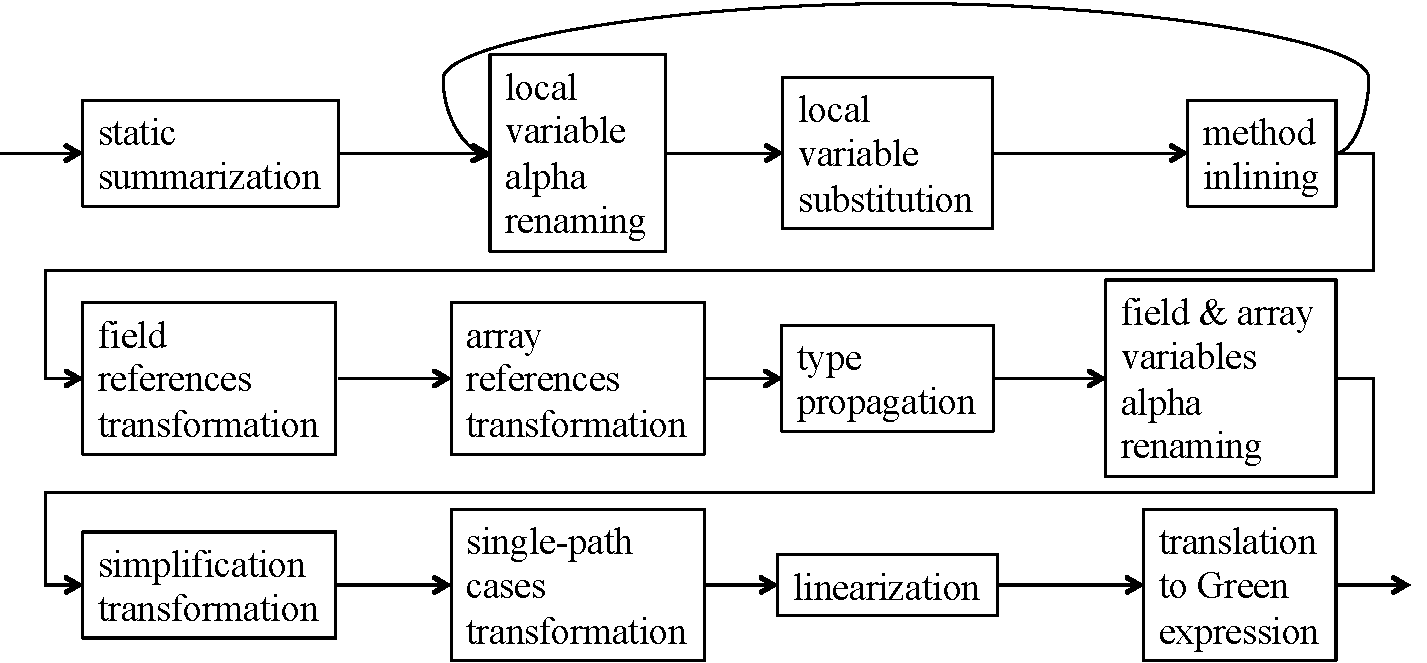
\includegraphics[width=\textwidth]{chapters/java_ranger/figures/overview.pdf}
\end{figure}
%
%
%\subsection{WALA-based analysis for veritesting}
%%
%Veritesting requires static construction of
%predicates of a multi-path region which represent changes to the path expression of the dynamic
%symbolic executor.
%%
%It also requires construction of a control-flow graph of method bodies
%from Java bytecode and finding exit points of the region, which in turn
%requires creation of a control-flow graph of the region.
%%
%Implementing veritesting is made simpler by using a static single
%assignment~(SSA)~\cite{ssa} representation of the multi-path region.
%%
%Using an SSA form allows us to use the $\phi$-expressions created by the
%SSA form and translate them into points at the end of the veritesting
%region where updates to system state along different paths in the region
%can be merged.
%%
%\mike{MWW: Vaibhav please update to describe WALA}
%WALA~\cite{} is a static analysis framework for Java programs that
%has both these features, with
%ExceptionalUnitGraph~\cite{exceptionalunitgraph} and the Shimple
%IR~\cite{shimple}.
%%
%For simple regions with only one exit point, like the one presented in Listing~\ref{lst:v_ex}, we
%were able to use Soot to automate static construction of the predicate representing
%an update to the expression.
%%
%For doing this, we used nodes with more than one successor as the
%starting point, found the immediate post-dominator of the starting
%point, and traversed the control-flow graph on all sides of such branches.
%%
%During such a traversal, we constructed predicates representing the
%multi-path region, similar to the ones presented in
%Listing~\ref{lst:v_ex_smt2}.
%%
%As explained in Section~\ref{sec:exit_points}, including virtual
%function invocations in the construction of our predicates amplifies the
%benefits of veritesting even further.
%%
%We plan to automate this inclusion in the future using Soot.
%%
%Providing SPF with updates to be made to its symbolic store also
%requires Soot to maintain stack location information for variables.
%%
%We plan to automate SPF\rq s symbolic store updates using Soot in the
%future.
%%
%

\subsection{Statement Recovery}
\label{sec:static-analysis}
%Java Ranger has its own AST that captures the statement of regions.
%%
%The choice of having a separate AST for Java Ranger, enables the integration of Java Ranger with any static analysis framework by implementing the transformation that transforms the CFG of a given IR into the corresponding Java Ranger AST representation. 
%%
%We call this interface \textit{Statement Recovery} transformation. \\
%%
%In this transformation we visit nodes in topological order by walking normal edges of a branching points until a \textit{minimum convergent node} is encountered. We define a minimum convergent node as the last immediate successor of blocks following a branching node.
%%
%Note that exceptional edges are ignored during this transformation, however exceptional behavior is later identified and handled through the single path cases.
%%
%We discuss more about this in section~\ref{sec:instantiationTransformations}.
%%
%There are two other things that this transformation takes care of: recovering of complex if-then-else and construction of Gated Single Assignment (GSA).
%%
%Recovering of complex conditions in an if-statement restores its form in the source code. 
%% 
%This is done by identifying \textit{immediate self-contained subgraphs}, that is, subgraphs where the initial node is immediately pre-dominated by the initial node and for the static region and whose successor nodes (up to the region terminus) are dominated (not necessarily immediately) by the initial node.
%%
%
%Construction of Gated Single Assignment (GSA) on the other hand is done by keeping track of the current "conditional path" during translation. More precisely this is done by keeping a stack of  {\tt(Expression x enum \{Then, Else\})} pairs. 
%%
%In addition to that, for each edge between blocks in the block structure, the associated "conditional path" is recorded.  
%%
%So the type of this map (the blockConditionMap) is: {\tt(ISSABasicBlock x ISSABasicBlock) --> List of (Expression x enum \{Then, Else\})}.
%%
%Finally creation of the condition of GSA is done during translating a phi-instruction its immediate predecessor blocks are retrieved then we look up  the edges in the blockConditionMap.  From here, and using condition stack leading to that branch, an if/then/else statement is constructed.

The regions of interest for our technique are bounded by the branch and meet of a given acyclic subgraph.  The intuition is that path explosion during execution of loops is driven by conditional logic within the loop, rather than the loop itself.
Starting from an SSA form, the first transformation recovers a tree-shaped AST for the subgraphs of interest.  While this step is not strictly necessary, it substantially simplifies subsequent transformations.  

The algorithms are similar to those used for those used for decompilation~\cite{Yakdan15@decompilation} but with slightly different goals: 
\begin{itemize}
    \item The algorithm must be {\em accurate} but need not be {\em complete}.  That is, obfuscated regions of code need not be translated into a tree form.
    \item The algorithm must be {\em lightweight} in order to be efficiently performed during analysis.  Thus, algorithms that use global fixpoint computations are 
        too expensive to be used for our purposes.
\end{itemize}

Starting from an initial SSA node, the algorithm first finds the immediate post-dominator of all {\em normal} control paths, that is, paths that do not end in an exception or return instruction.  It then looks for nested self-contained subgraphs.  If for any graph, the post-dominator is also a predecessor of the node, we consider it a loop and discard the region.  

The algorithm systematically attempts to build regions for every branch instruction, even if the branch is already contained within another region.  The reason is that it may not be possible to instantiate the larger region depending on whether summaries can be found for {\em dynamically-dispatched} functions, and whether references are {\em uniquely determinable} for region outputs.

\iffalse
\begin{verbatim}

stmt ::= stmt ; 
   

\end{verbatim}

\vaibhav{assigned to Mike}
\mike{MWW: - we should provide an AST of the constraint language}
\fi 

\subsection{Region Definition}

Once the statement of a multi-path region has been recovered, its corresponding environment is populated.
%
This includes identifying region boundary and creating local variable inputs, outputs, type, and stack slot tables for
the region.
%
The region boundary is used to identify boundaries of the region w.r.t local variables.
%
This is used later to constrain the computation and population of Ranger IR environment tables.
%
For example, the local variable input table is populated with first \textit{use} in the region boundary that map to a given stack slot.
%
The output table is populated with the last \textit{def} of a local variable at merge point of the region.
%
The local variable type table is populated for all variables that lay within the boundaries of the region, this is initially done by
inquiring the static analysis framework, WALA~\cite{Wala} but is later changed by inferring types of local variables
at instantiation and during type propagation transformation~\ref{sec:instantiationTransformations}.

We also construct a stack slot table as part of a region\rq s Ranger IR summary.
%
The stack slot table maps Ranger IR variables to a stack slot, if they correspond to a local variable in the source code.
%
We populate the stack slot table by obtaining a variable to stack slot mapping from WALA.
%
We also assume that, if at least one variable used in a $\phi$-expression is a local variable, then all variables
used in that $\phi$-expression must belong to the same stack slot.
%
We use this assumption to further propagate stack slot information in the stack slot table across all $\phi$-expressions
encountered at merge points of regions.

%The stack slot table on the other hand, does not use region boundary for its population. The reason for this is that,
%the static analysis framework we use, WALA, sometime does not provide information about the stack slots of intermediate
%variables.
%%
%This is particularly problematic in our case because the def of a phi is both an intermediate variable, and so we do
%not know its stack slot, yet it is also an output of the region for which we want to populate its symbolic
%representation onto the stack slot.
%%
%Therefore, our stack slot table uses stack slot inference by propagating the stack slots of vars used in a phi onto the
%def of the phi.
%%
%This requires visiting all variables and phi statements of the IR to maximize the inference of the stack slot, this is
%repeatedly done until a fix point is reached.


\subsection{Instantiation-time Transformations}
\label{sec:instantiationTransformations}

\textbf{Renaming Transformation}: In Alpha renaming transformation, all Ranger IR variables are renamed to ensure their uniqueness before further processing takes place. 
%
This is particularly important not only to ensure uniqueness of variables among different regions, but also to ensure
uniqueness of variable names of the \textit{same} region which might be instantiated multiple times on the same path,
i.e., a region inside a loop will be instantiated multiple times.\\
%
\textbf{Local Variable Substitution Transformation}: During this transformation we eagerly bring in all dynamically
known constant values, symbolic values and references from stack slots into the region for further processing. \\
%
\textbf{Higher-order Regions Transformation}: This transformation is initiated when a method invocation is encountered
during local variable substitution.
%
At this point, we perform three steps.
%
(1) the region that corresponds to the called method is retrieved and alpha renaming of
Ranger IR variables corresponding to local variables is applied on it.
%
(2) Ranger IR expressions that correspond to the actual parameters are evaluated and used to substitute the formal
parameters by repeatedly applying local variable substitution transformation over the method region.
%
(3) When no more higher-order regions can be inlined, the resulting substituted method region is inlined into
the outer region.\\
%
If the method region has a single return value, then the original method invocation is replaced with an assignment to
the returned expression.
%
%Otherwise, inlining of the method region takes place.
%
We dont currently support instantiation of method regions with multiple return statements, support for which requires
another transformation that we talk about in Section~\ref{sec:future}.
\\
\textbf{Field References SSA form}: The field references transformation translates reads and writes of fields
in Java bytecode into corresponding Ranger IR statements.
%
In order to translate all field accesses to SSA form, this transformation creates a summary of the semantics
represented by the field accesses in the region.
%
This transformation constructs a new field access variable for every field assignment on every path within the region.
%
This new field access variable construction makes use of two monotonically increasing subscripts.
%
It uses a path subscript to distinguish between assignments to the same field on the same execution path.
%
It uses a global subscript to distinguish between assignments to the same field across execution paths.
%
At the merge point of the region, field assignments done on the same field are merged using
Gated Single Assignment (GSA)~\cite{Ottenstein1990}.
%
Each merged field access variable has its own path and global subscripts and represents the output of the region into
its field.
%
The path subscript helps us resolve read-after-write operations on the same execution path and find the latest write
into a field on an execution path.
%
The global subscript helps us distinguish between field accesses across multiple execution paths. \\
\textbf{Array References SSA form}: The array references transformation translates reads and writes of arrays in
Java bytecode into corresponding Ranger IR statements.
%
In order to translate all array accesses to SSA form, this transformation creates an execution path-specific copy of
every array when it is first accessed within a region.
%
Reads and writes of arrays are then done on a path-specific copy of the array.
%
All array copies are merged at the merge point of multi-path regions.
%
The merged array copy represents array outputs of the region.\\
\textbf{Type Propagation}: Ranger IR needs to have type information for its variables so that it can construct
corresponding correctly-typed Green variables during the final transformation of the region summary to a Green formula.
%
Having accurate type information is also important for looking up the correct higher-order method summary.
%
As part of region instantiation, Java Ranger infers types of Ranger IR variables in the region summary by
using JPF's runtime environment.
%
Types of local variables are inferred during the local variable substitution transformation and types of field reference
and array reference variables are inferred during their respective transformations.
%
Using these inferred types, the type propagation transformation propagates type information across assignment
statements, binary operations, and variables at leaf nodes of $\gamma$ functions.\\
%
\textbf{Simplification of Ranger IR}: The Ranger IR constructed by earlier transformations computes exact semantics
of all possible behaviors in the region.
%
Representation of such semantics as a formula can often lead to unnecessarily large formulas, which has the potential to
reduce the benefits seen from path merging~\cite{angr}.
%
For example, if an entry in an array is never written to inside a region, the array reference transformation can still have an
array output for that entry that writes a new symbolic variable into it.
%
The region summary would then need to have an additional constraint that makes the new symbolic variable equal the
original value in that array entry.
%
Such conjuncts in the region summary can be easily eliminated with constant propagation, copy propagation, and constant
folding~\cite{dragon-book}.
%
Ranger IR also has statement and expression classes that use a predicate for choosing between two statements (similar to
an {\tt if} statement in Java) and two sub-expressions (similar to the C ternary operator) respectively.
%
When both choices are syntactically equal, the predicated statement and expression objects can be substituted with the
statement or expression on one of their two choices.
%
Such statements and expressions were simplified away to use one of their two choices.
%
Ranger IR performs these two simplifications on such predicated statements and expressions along with constant folding,
constant propagation, and copy propagation.\\
\textbf{Single Path Cases}: This transformation collects path predicates inside a region that lead to
\textit{non-nominal} exit point.
%
This is an alternative approach to that was presented in \cite{veritesting}.
%
In our work we define non-nominal exit point to be points inside the region that either define exceptional behavior or
involve behavior that we cannot summarize, i.e, object creation and throw instructions.
%
The intuition here is that, we want to maximize regions that Java Ranger can summarize, even if the summarization is
only partial.
%
We use this pass of transformation to identify such points, collect their path predicates and prune them away from the
Ranger IR statement.
%
The outcome of this process, is a more simplified and concise statement that represent the nominal behavior of the Ranger region.
%
The collected predicate is later used to guide the symbolic execution to explore non-nominal paths, which Java Ranger
had not summarized.  \\
%
\textbf{Linearization}:
Ranger IR contains translation of branches in the Java bytecode to if-then-else statements defined in the Ranger IR.
%
But the if-then-else statement structure needs to be kept only as long as we have more GSA expressions to be
introduced in the Ranger IR.
%
Once all GSA expressions have been computed, the Ranger IR need not have if-then-else statements anymore.
%
The $\gamma$ functions introduced by GSA are a functional representation of branching, which lets us
capture the semantics of everything happening on both sides of the branch.
%
Since the linearization transformation is done after every field and array entry has been unaliased and converted to
GSA, dropping if-then-else statements from the Ranger IR representation of the region summary reduces redundancy in its
semantics and converts it into a stream of GSA and SSA statements.\\
\textbf{Translation to Green}:
%
At this point Ranger region contains only compositional statements as well as assignment statements that might contain GSA expressions in them.
%
This transformation starts off by translating Ranger variables to Green variables of the right type using the region type table.
%
Then Ranger statements are translated. More precisely, compositional statements are translated into conjunction, assignment statements are translated into Green equality expressions.
%
For assignment statements that have GSA expressions, these are translated into two disjunctive formulas that describes the assignment if the GSA condition or its negation were satisfied.

The sequence in which these Ranger IR transformations are performed should not matter.
%
This sequence of transformations should be run up to a fixed point so that we can have resolve local
variable, field, and array inputs in an arbitrary order, as was seen with the motivating example described in Figure~\ref{fig:mot-example}.
%
Currently Java Ranger does not support such a fixed point computation, but we plan to automate this computation in the future.

\subsection{Checking Correctness Of Region Summaries}
The Ranger IR computed as a result of performing the transformations described in Figure~\ref{fig:overview} should
correctly represent the semantics of the summarized region.
%
If it does not, then using the instantiated region summary can cause symbolic exploration to explore the wrong behavior
of the subject program.
%
We checked the correctness of our instantiated region summaries by using equivalence-checking as defined by Ramos et al.~\cite{ramos}.
%
We designed a test harness that first executes the subject program with a set of symbolic inputs using SPF and
capture the outputs of the subject program.
%
Next, the test harness executes the same subject program with the same set of symbolic inputs using Java Ranger and
capture the outputs of the subject program once again.
%
Finally, the test harness compares outputs returned by symbolic execution with SPF and Java Ranger.
%
If the outputs do not match, then a region summary used by Java Ranger did not contain all the semantics
of the region it summarized.
%
We symbolically execute all execution paths through this test harness.
%
If no mismatch is found between outputs on any execution path, we conclude that all region summaries used by Java Ranger
must correctly represent the semantics of the regions they summarized.
%
We performed correctness-checking on all results reported in this paper.

%\input{experiments}
\section{Evaluation}
\label{sec:results}
\subsection{Experimental Setup}
We implemented the above mentioned transformations as a wrapper around the Symbolic PathFinder~\cite{spf} tool.
%
To make use of region summaries in Symbolic PathFinder, we use an existing feature of SPF named \textit{listener}.
%
A listener is a method defined within SPF that is called for every bytecode instruction executed by SPF.
%
Java Ranger adds a path merging listener to SPF that, on every instruction, checks (1) if the instruction involves
checking a symbolic condition, and (2) if Java Ranger has a pre-computed static summary that begins at that
instruction\rq s bytecode offset.
%
If both of these conditions are satisfied, Java Ranger instantiates the multi-path region summary corresponding to that
bytecode offset by reading inputs from and writing outputs to the stack and the heap.
%
It then conjuncts the instantiated region summary with the path condition and resumes symbolic execution at the
bytecode offset of the end of the region.
%
Our implementation, named Java Ranger, wraps around SPF and can be configured to run in four modes.
%
(1) In mode 1, it runs vanilla SPF without any path merging enabled.
%
(2) In mode 2, it summarizes multi-path regions only and instantiates them if they are encountered.
%
(3) In mode 3, it summarizes and instantiates methods, by utilizing high ordder regions, along with multi-path regions
as done in mode 2.
%
(4) In mode 4, it uses single-path cases along with multi-path region and method summaries used in mode 3.
%
\subsection{Evaluation}
%\input{static-analysis-results}
\input{chapters/java_ranger/results-big-table}
%
In order to evaluate the performance of Java Ranger, we used the following benchmarking programs commonly used to evaluate symbolic
execution performance.
%
(1) Wheel Brake System (WBS)~\cite{yang2014directed} is a synchronous reactive
component developed to make aircraft brake safely when taxing, landing, and during a rejected take-off.
%
(2) Traffic Collision Avoidance System (TCAS) is part of a suite of programs commonly referred to as the Siemens
suite~\cite{siemens-benchmarks}. TCAS is a system that maintains altitude separation between aircraft to avoid mid-air
collisions.
%
(3) Replace is another program that\rq s part of the Siemens suite. Replace searches for a pattern in a given input and
replaces it with another input string.
%
We used the translation of the Siemens suite to Java as made available by Wang et al.~\cite{dgse}.
%
We also manually created a variant of TCAS by converting regions of code with return statements on
every execution path to regions of code with a single return statement at the merge point of the region.
%
We refer to this variant of TCAS as TCAS-SR (TCAS with Single Returns).
%
We also created variants of WBS, TCAS, and TCAS-SR by running them for multiple steps.
%

%We ran WBS, TCAS, TCAS-SR, and Replace using Java Ranger and first report the result of static analysis on these
%three benchmarks in Table~\ref{table:static-analysis}.
%
%The number of static regions summarized for WBS and TCAS is dominated by region summaries found in the Java standard
%library used by WBS and TCAS.
%%
%Replace doesn't use the Java standard library, which is reflect in Table~\ref{table:static-analysis}.
%%
%We also report the most number of branches seen in our static regions with each benchmark.
%%
%Being able to instantiate static summaries of such regions potentially increases the path reduction we get from path-merging.

We ran WBS, TCAS, TCAS-SR, and Replace using Java Ranger and present our results from instantiating region summaries
in Table~\ref{table:results}.
%
Table~\ref{table:results} shows that Java Ranger achieves a significant improvement using path-merging with WBS.
%
The ``\# exec paths'' column is the number of execution paths required to completely explore the benchmark.
%
``runtime (msec)'' is the time taken for dynamic analysis (excludes static analysis time).
%
``\# inst. regs'' is the total number of regions that were instantiated at least once when running each benchmark.
%
``\# inst. methods'' is the number of higher-order regions that were used and ``inst.'' is the total number of
instantiations that was done when running the benchmark.
%
Table~\ref{table:results} shows that we achieve a significant improvement using path-merging with WBS.
%
Java Ranger outperforms SPF when running TCAS too but it doesn't allow path merging to summarize the entire program
to a single execution path, as in the case with WBS.
%
We manually analyzed TCAS and found the only barrier to our path-merging was the presence of several code
regions containing a return instruction on every execution path.
%
We manually performed a semantics-preserving transformation to the source code of TCAS to create another version, TCAS-SR,
that has a single return value at the end of all such multi-path regions.
%
We plan to automate this transformation in the future, see future work section~\ref{sec:futureWork}.
%
Table~\ref{table:results} shows the benefit of such a \textit{multiple-returns-to-single-return} transformation.
%
It allows Java Ranger to summarize the entire TCAS-SR program into a single execution path.
%
This is made possible by the use of higher-order regions as shown in Table~\ref{table:results}.
%
In mode 2, Java Ranger explores 18 execution paths with TCAS-SR, whereas in mode 3~(mode 2 + higher-order region support), it needs to only explore a single
execution path because it can instantiate 28 higher-order method summaries.
%
The bottom half of Table~\ref{table:results} also shows the benefits of path-merging with Java Ranger increase as we run
more steps of WBS, TCAS, and TCAS-SR.
%
We ran as many steps of each of these 3 benchmarks as possible with a 6 hour timeout using Java Ranger in modes
1 (runs Java Ranger without path merging) and 3 (runs Java Ranger with multi-path region summaries and higher-order region summaries).
%
While, in mode 1, Java Ranger can only run 5 steps of WBS in less than 6 hours, in mode 4 (path merging with multi-path regions, higher-order regions, and single-path cases),
Java Ranger can easily execute up to 10 steps in less than 4 seconds.
%
A similar benefit is seen with TCAS-SR where Java Ranger in mode 1 can only run 2 steps of TCAS-SR in 6 hours, but in
mode 4, it can easily run up to 10 steps of TCAS-SR in about 1 second.

However, the performance of Java Ranger when running Replace is quite different from that seen when running WBS, TCAS, and TCAS-SR.
%
While Java Ranger reduces the total number of execution paths with every increase in mode, the path reduction isn't as significant.
%
More importantly, it also makes an order of magnitude more solver calls thereby increasing the total runtime.

We further investigated this drop in performance of Java Ranger when running Replace by exploring the space of potential
regions to instantiate.
%
We obtained the list of regions that are instantiated at least once when running Replace with Java Ranger in mode 3~(using
high order and multi-path region summaries).
%
This step produced a list of 24 regions.
%
Next, we sampled the space of all possible subsets of this set of 24 regions by
%
(1) randomly enumerating the space up to 11500 subsets of all possible subsets of 24 regions,
%
(2) enumerating the space in the order of set size up to all subsets of 3 regions from a set of 24 regions.
%
With both methods of enumeration, we searched for the least amount of time Java Ranger needs to instantiate at least one
region with Replace.
%
We found this least time to be 26.3 seconds which is still more than the 3.47 seconds Java Ranger needs to run
Replace in mode 1 (running vanilla SPF with no path merging).
%
In the fastest runs with at least one region instantiation in both methods of enumeration, Java Ranger finished
exploration with the same number of execution paths as that explored during mode 1.
%
The result of this analysis, combined with a significant increase in the number of solver queries with Java Ranger's
path-merging modes, points toward the conclusion that every instantiation of a multi-path region in Replace causes another branch to be
symbolic.
%
This conclusion is also in alignment with the observation made by Kuznetsov et al.~\cite{kuznetsov} that path merging can
sometimes have a net negative effect on the performance of symbolic execution.
%
We plan to integrate heuristics for estimating the side-effects of introducing new symbolic state as a result of
path merging on symbolic execution performance with Java Ranger in the future.

\section{Future Work}
\label{sec:futureWork}
While Java Ranger has the potential to scale to large real-world Java programs, there are a number of directions along
which it can be further improved.
\begin{itemize}

\item Java Ranger attempts to perform path merging as aggresively as possible. This path merging strategy doesn't
optimize towards making fewer solver calls. We plan to work towards implementing heuristics that
can measure the effect of path merging on the rest of the program.
    
%\item In some models, it is possible to reduce the number of paths to one.  The static region approach essentially
%constructs a unrolled version of the program, similar to what tools like CBMC construct.   This can only happen on
%relatively static models that do not have a lot of object construction leading to multiple dispatch paths.  HOSRs are
%more flexible for these situations and allow specialization depending on dispatch type, which we believe will lead to
%better performance for highly-dynamic models.
%
%\item In general, the solver time does not rise dramatically for disjunctive paths. Since (in the limit) we reduce the
%number of paths exponentially by removing branches, we can perform relatively expensive analyses as preprocessing steps
%and at instantiation if we are able to instantiate a static region, and still end up with much better performance.

\item Java Ranger is most useful when it can merge multiple execution paths into one summary. But such merging causes an
increase in the size of the summary, and consequently, the path condition.
%
Once a summary has been communicated to the solver, it need not be sent again as long as it remains the same.
%
This requires us to use the solver in an incremental mode, where we use previously-constructed state in the solver for
future solving.
%
Our current implementation of Java Ranger sends the entire path condition to the solver with every query, making every
query even more expensive in the presence of large multi-path region summaries.
%
We plan to integrate incremental solving with Java Ranger in the future.
%
\item Multiple return instructions that appear on all execution paths inside a multi-path region can be simplified to a
single return value of the region.
%
We implemented this transformation manually in TCAS but we plan to automate it in the future.
%
Such automation would allow us to summarize regions with return instructions.
%
\item While statically summarizing regions gives dynamic symbolic execution a
performance boost to explore more paths efficiently, generating test cases that covers all summarized branches is one of
the fundamental roles of dynamic symbolic execution that is currently unsupported.
%
This is an extension that we intend to investigate in our future work.
%
\item While path merging can potentially allow symbolic execution to explore interesting parts of a program sooner, the
effect of path merging on search strategies, such as depth-first search and breadth-first search commonly used with
symbolic execution, remains to be investigated. We plan to explore the integration of such guidance heuristics with path merging in the future.
%
\item Java Ranger can summarize methods and regions in Java standard libraries. This creates potential for automatically
constructing summaries of standard libraries so that Java symbolic execution engines can prevent path explosion
originating from standard libraries.
%
\end{itemize}
\section{Conclusion}
\label{sec:future}

We presented Java Ranger as a path merging tool for Java.
%
It works by systematically applying a series of transformations over a statement recovered from the CFG. This
representation provides the benefit of modularity and makes path-merging for Java symbolic execution more accessible to
end users.
%
Java Ranger has its own IR statement and it supports the construction of SSA for fields and arrays.
%
Java Ranger provides evidence that inlining summaries of higher-order regions can lead to a further reduction in the
number of execution paths that need to be explored with path merging.
%
It supports the exploration of exceptional behavior in multi-path regions via Single Path Cases which is an alternative
technique for summarizing unexceptional behavior while simultaneously capturing exceptional behavior of a region.
%
Java Ranger reinterprets path merging for symbolic execution of Java bytecode and has the potential to allow symbolic
execution to scale up to exploration of real-world Java programs.





%%%%%%%%%%%%%%%%%%%%%%%%%%%%%%%%%%%%%%%%%%%%%%%%%%%%%%%%%%%%%%%%%%%%%%%%%%%%%%%%

%%%%%%%%%%%%%%%%%%%%%%%%%%%%%%%%%%%%%%%%%%%%%%%%%%%%%%%%%%%%%%%%%%%%%%%%%%%%%%%%
% program_repair.tex:
%%%%%%%%%%%%%%%%%%%%%%%%%%%%%%%%%%%%%%%%%%%%%%%%%%%%%%%%%%%%%%%%%%%%%%%%%%%%%%%%
\chapter{Program Repair Using Adapter Synthesis}
\label{program_repairn_chapter}
%%%%%%%%%%%%%%%%%%%%%%%%%%%%%%%%%%%%%%%%%%%%%%%%%%%%%%%%%%%%%%%%%%%%%%%%%%%%%%%%

%%%%%%%%%%%%%%%%%%%%%%%%%%%%%%%%%%%%%%%%%%%%%%%%%%%%%%%%%%%%%%%%%%%%%%%%%%%%%%%%


%Analysis Chapters
%\include{chapters/data_set}
%\include{chapters/event_selection}
%\include{chapters/analysis}

%Conclusion
\section{Conclusion}
\label{sec:future}

We presented Java Ranger as a path merging tool for Java.
%
It works by systematically applying a series of transformations over a statement recovered from the CFG. This
representation provides the benefit of modularity and makes path-merging for Java symbolic execution more accessible to
end users.
%
Java Ranger has its own IR statement and it supports the construction of SSA for fields and arrays.
%
Java Ranger provides evidence that inlining summaries of higher-order regions can lead to a further reduction in the
number of execution paths that need to be explored with path merging.
%
It supports the exploration of exceptional behavior in multi-path regions via Single Path Cases which is an alternative
technique for summarizing unexceptional behavior while simultaneously capturing exceptional behavior of a region.
%
Java Ranger reinterprets path merging for symbolic execution of Java bytecode and has the potential to allow symbolic
execution to scale up to exploration of real-world Java programs.



%%%%%%%%%%%%%%%%%%%%%%%%%%%%%%%%%%%%%%%%%%%%%%%%%%%%%%%%%%%%%%%%%%%%%%%%%%%%%%%%

%%%%%%%%%%%%%%%%%%%%%%%%%%%%%%%%%%%%%%%%%%%%%%%%%%%%%%%%%%%%%%%%%%%%%%%%%%%%%%%%
% Bibliography
%%%%%%%%%%%%%%%%%%%%%%%%%%%%%%%%%%%%%%%%%%%%%%%%%%%%%%%%%%%%%%%%%%%%%%%%%%%%%%%%
%\bibliography{thesis}
\bibliography{chapters/adapter_synthesis/references,chapters/java_ranger/references}
%%%%%%%%%%%%%%%%%%%%%%%%%%%%%%%%%%%%%%%%%%%%%%%%%%%%%%%%%%%%%%%%%%%%%%%%%%%%%%%%

%%%%%%%%%%%%%%%%%%%%%%%%%%%%%%%%%%%%%%%%%%%%%%%%%%%%%%%%%%%%%%%%%%%%%%%%%%%%%%%%
% Appendices
%%%%%%%%%%%%%%%%%%%%%%%%%%%%%%%%%%%%%%%%%%%%%%%%%%%%%%%%%%%%%%%%%%%%%%%%%%%%%%%%
\appendix
%\include{chapters/app_glossary}
%\section{Appendix}
\label{sec:appendix}




%

%%%%%%%%%%%%%%%%%%%%%%%%%%%%%%%%%%%%%%%%%%%%%%%%%%%%%%%%%%%%%%%%%%%%%%%%%%%%%%%%

%%%%%%%%%%%%%%%%%%%%%%%%%%%%%%%%%%%%%%%%%%%%%%%%%%%%%%%%%%%%%%%%%%%%%%%%%%%%%%%%
% End the Document
%%%%%%%%%%%%%%%%%%%%%%%%%%%%%%%%%%%%%%%%%%%%%%%%%%%%%%%%%%%%%%%%%%%%%%%%%%%%%%%%
\end{document}
%%%%%%%%%%%%%%%%%%%%%%%%%%%%%%%%%%%%%%%%%%%%%%%%%%%%%%%%%%%%%%%%%%%%%%%%%%%%%%%%
